\chapter{Appendix}
%% change chapter title to german if necessary
%% *** local page settings ***
\markright{Appendix}
\addtocontents{toc}{\protect\setcounter{tocdepth}{-1}} %decrease the depth of the appendix entry in the ToC
\setcounter{table}{0}
\setcounter{figure}{0}
\renewcommand{\thefigure}{A.\arabic{figure}}
\renewcommand{\thetable}{A.\arabic{table}}


\section{Further Model Constraints}

\begin{flalign}
	\label{parkCon_Q^{rB}_{DA}(t_{hour})}                   \sum((s_DA, s^{in}_{RL}, s^{out}_{RL}), Q^{rB}_{DA}(t_{hour}, s^{in}_{RL}, s^{out}_{RL})) \leq parkCap * parkProfile(t_{hour}) - \sum((s_DA, s^{in}_{RL}, s^{out}_{RL}), Q_rB_reload(t_{hour}, s^{in}_{RL}, s^{out}_{RL}));
\end{flalign}
\begin{flalign}
	\label{parkCon_Q^{rI}_{DA}(t_{hour})}                   \sum((s_DA, s^{in}_{RL}, s^{out}_{RL}), Q^{rI}_{DA}(t_{hour}, s^{in}_{RL}, s^{out}_{RL})) \leq parkCap * parkProfile(t_{hour}) - \sum((s_DA, s^{in}_{RL}, s^{out}_{RL}), Q_rI_reload(t_{hour}, s^{in}_{RL}, s^{out}_{RL}));
\end{flalign}
\begin{flalign}
	\label{parkCon_Q^{rO}_{DA}(t_{hour})}                   \sum((s_DA, s^{in}_{RL}, s^{out}_{RL}), Q^{rO}_{DA}(t_{hour}, s^{in}_{RL}, s^{out}_{RL})) \leq parkCap * parkProfile(t_{hour}) - \sum((s_DA, s^{in}_{RL}, s^{out}_{RL}), Q_rO_reload(t_{hour}, s^{in}_{RL}, s^{out}_{RL}));
\end{flalign}
\begin{flalign}
	\label{parkCon_Q^{rN}_{DA}(t_{hour})}                   \sum((s_DA, s^{in}_{RL}, s^{out}_{RL}), Q^{rN}_{DA}(t_{hour}, s^{in}_{RL}, s^{out}_{RL})) \leq parkCap * parkProfile(t_{hour}) - \sum((s_DA, s^{in}_{RL}, s^{out}_{RL}), Q_rN_reload(t_{hour}, s^{in}_{RL}, s^{out}_{RL}));
\end{flalign}
\section{Quantile Market Data}

\begin{figure}[!h]
	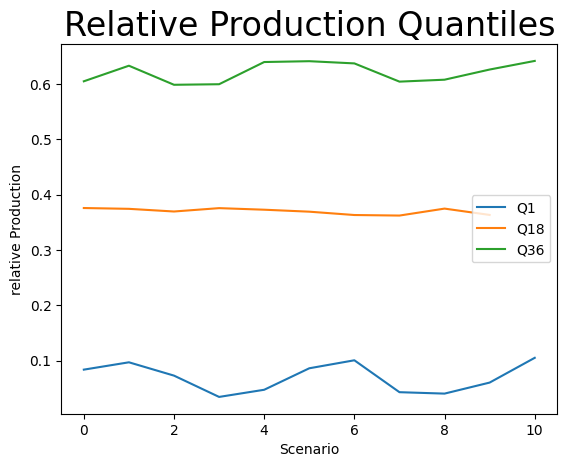
\includegraphics[width=0.7\linewidth]{pictures/results/relativeProduktionQuantils.png}
	\caption{Relative Production Quantiles}
	\label{fig:Relative Production Quantiles}
\end{figure}

Die daraus Resultierenden Zeitreihen für aktivierte Regelarbeit und deren Preise stellen sich dann wie folgt dar:
\begin{figure}[H]
	\centering

	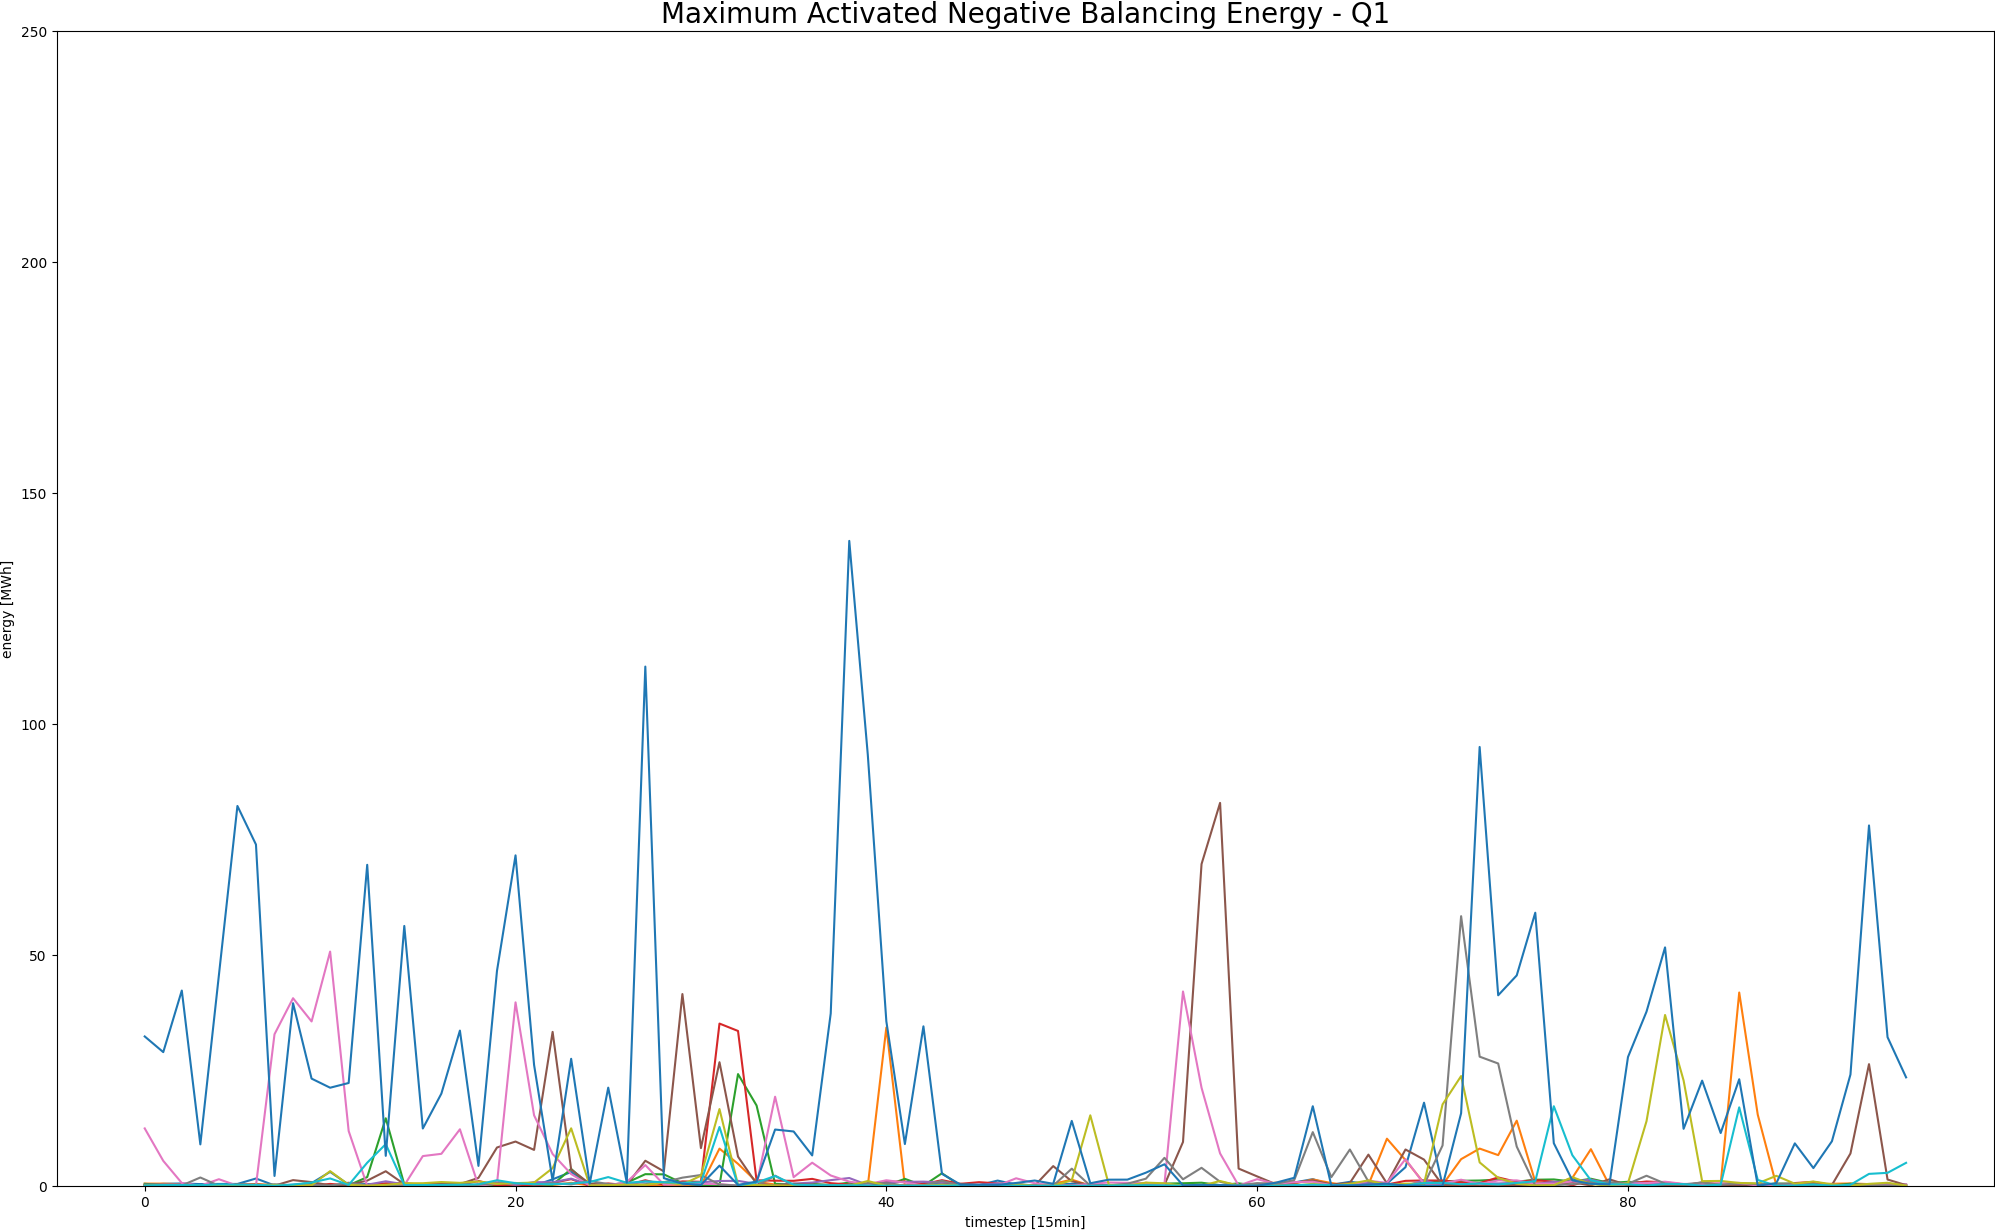
\includegraphics[width=1\linewidth]{pictures/results/Activated_negEnergy_Q1.png}
	\caption{Activated Negative Energy Q1}
	\label{fig:_negEnergy_Q1}
\end{figure}


\begin{figure}[H]
	\centering
	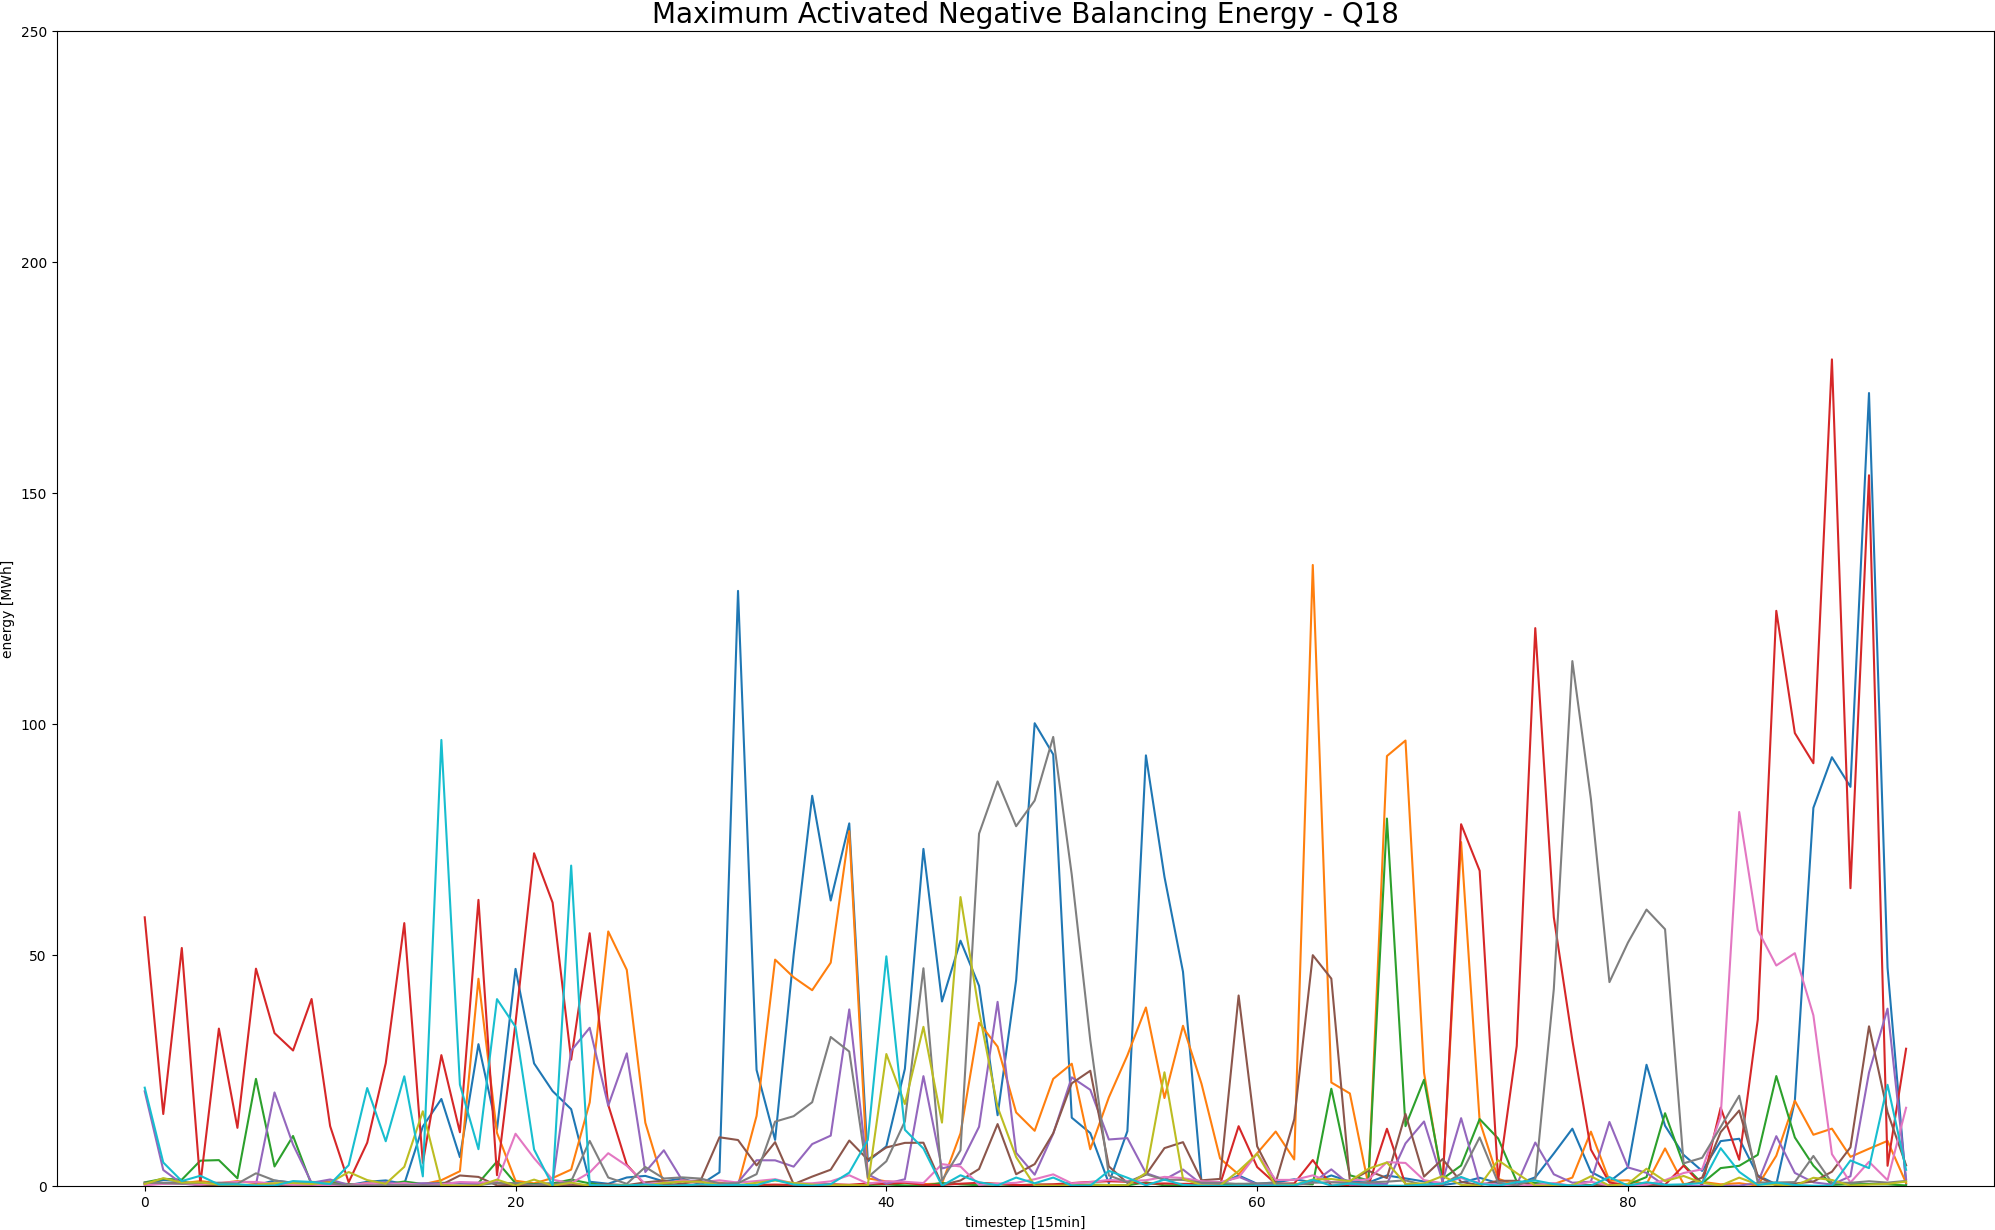
\includegraphics[width=1\linewidth]{pictures/results/Activated_negEnergy_Q18.png}
	\caption{Activated Negative Energy Q18}
	\label{fig:_negEnergy_Q18}
\end{figure}

\begin{figure}[H]
	\centering
	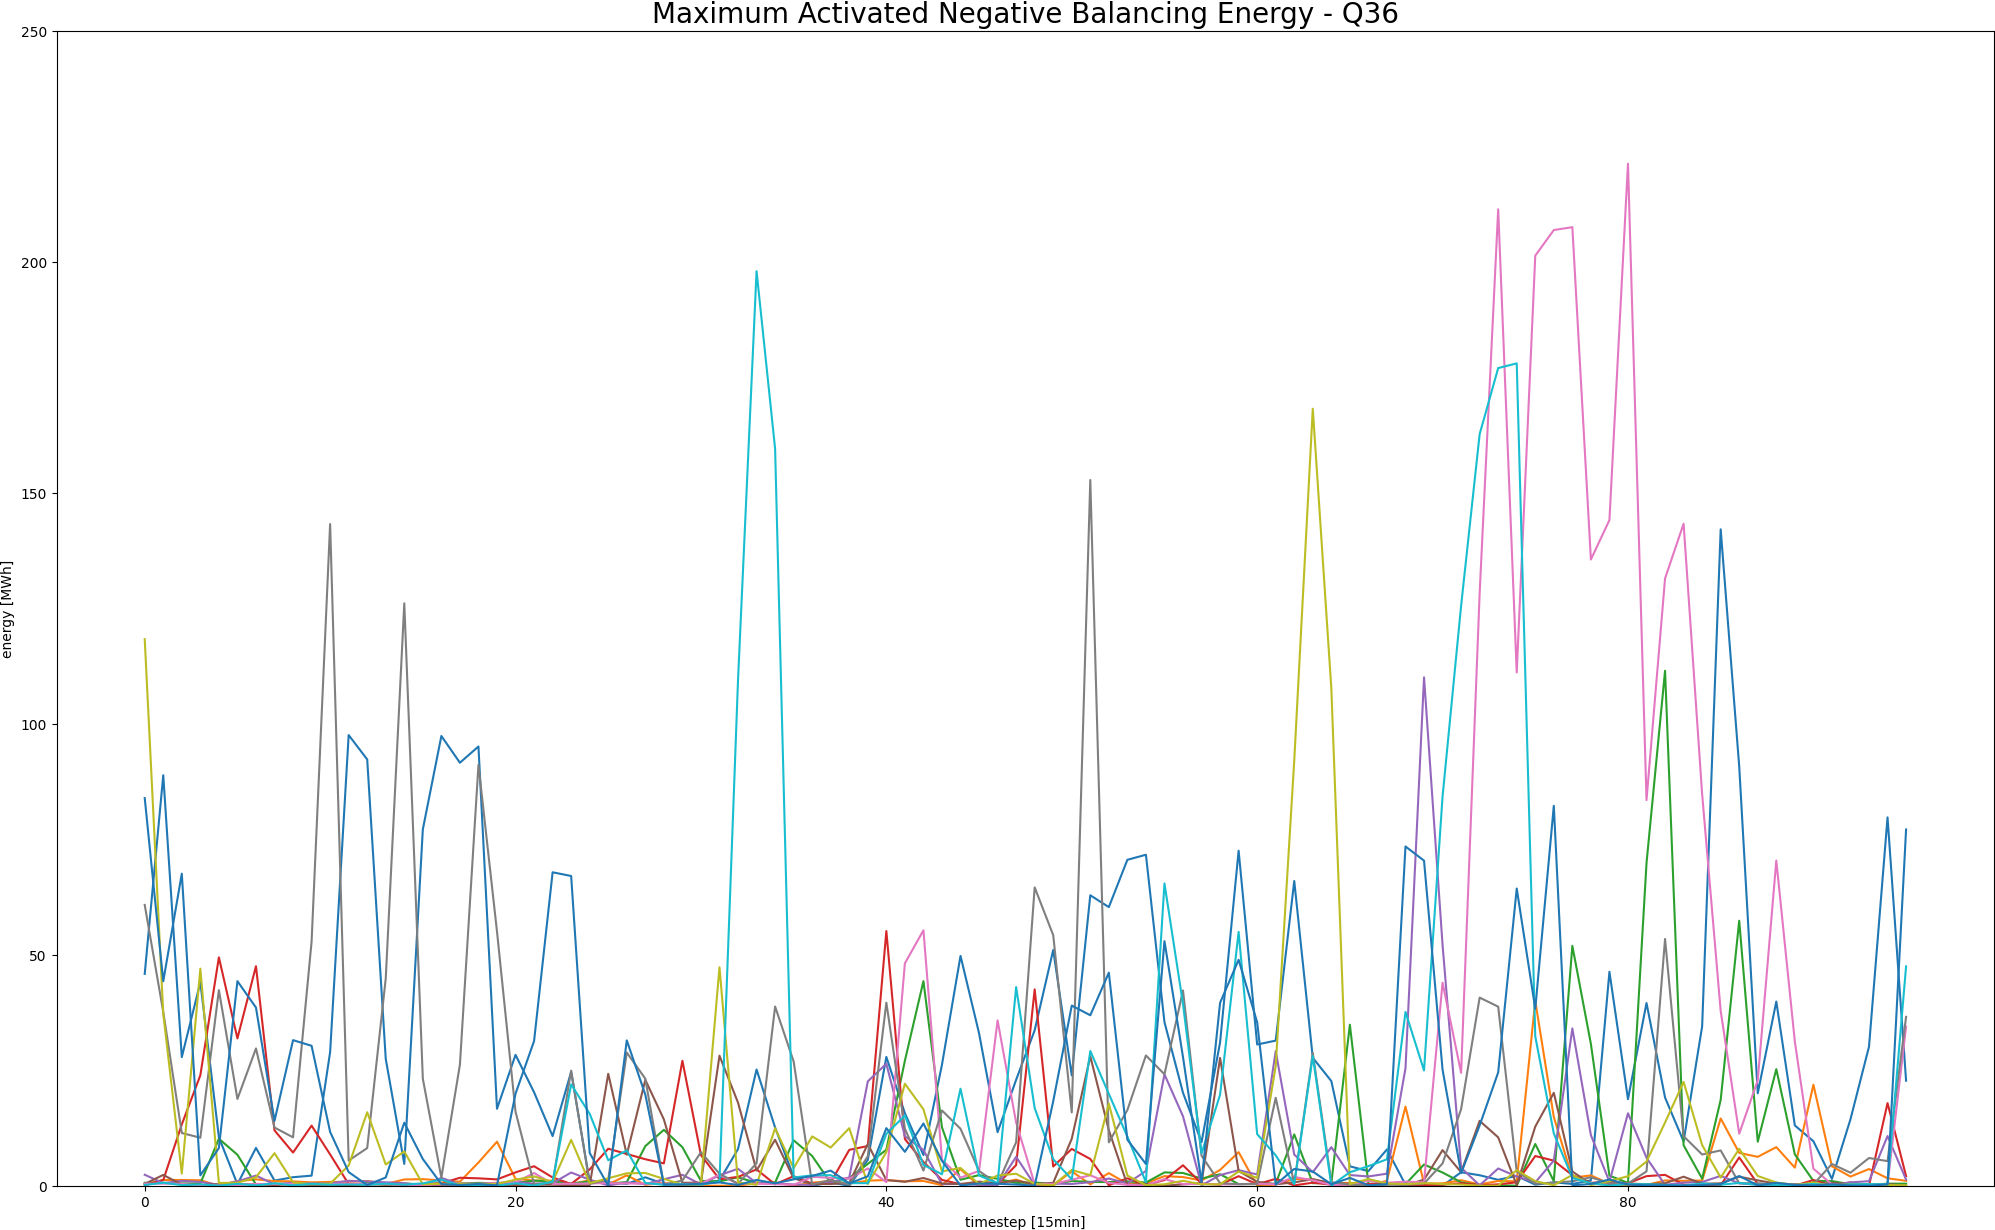
\includegraphics[width=1\linewidth]{pictures/results/Activated_negEnergy_Q36.png}
	\caption{Activated Negative Energy Q36}
	\label{fig:_negEnergy_Q36}
\end{figure}
\begin{figure}
	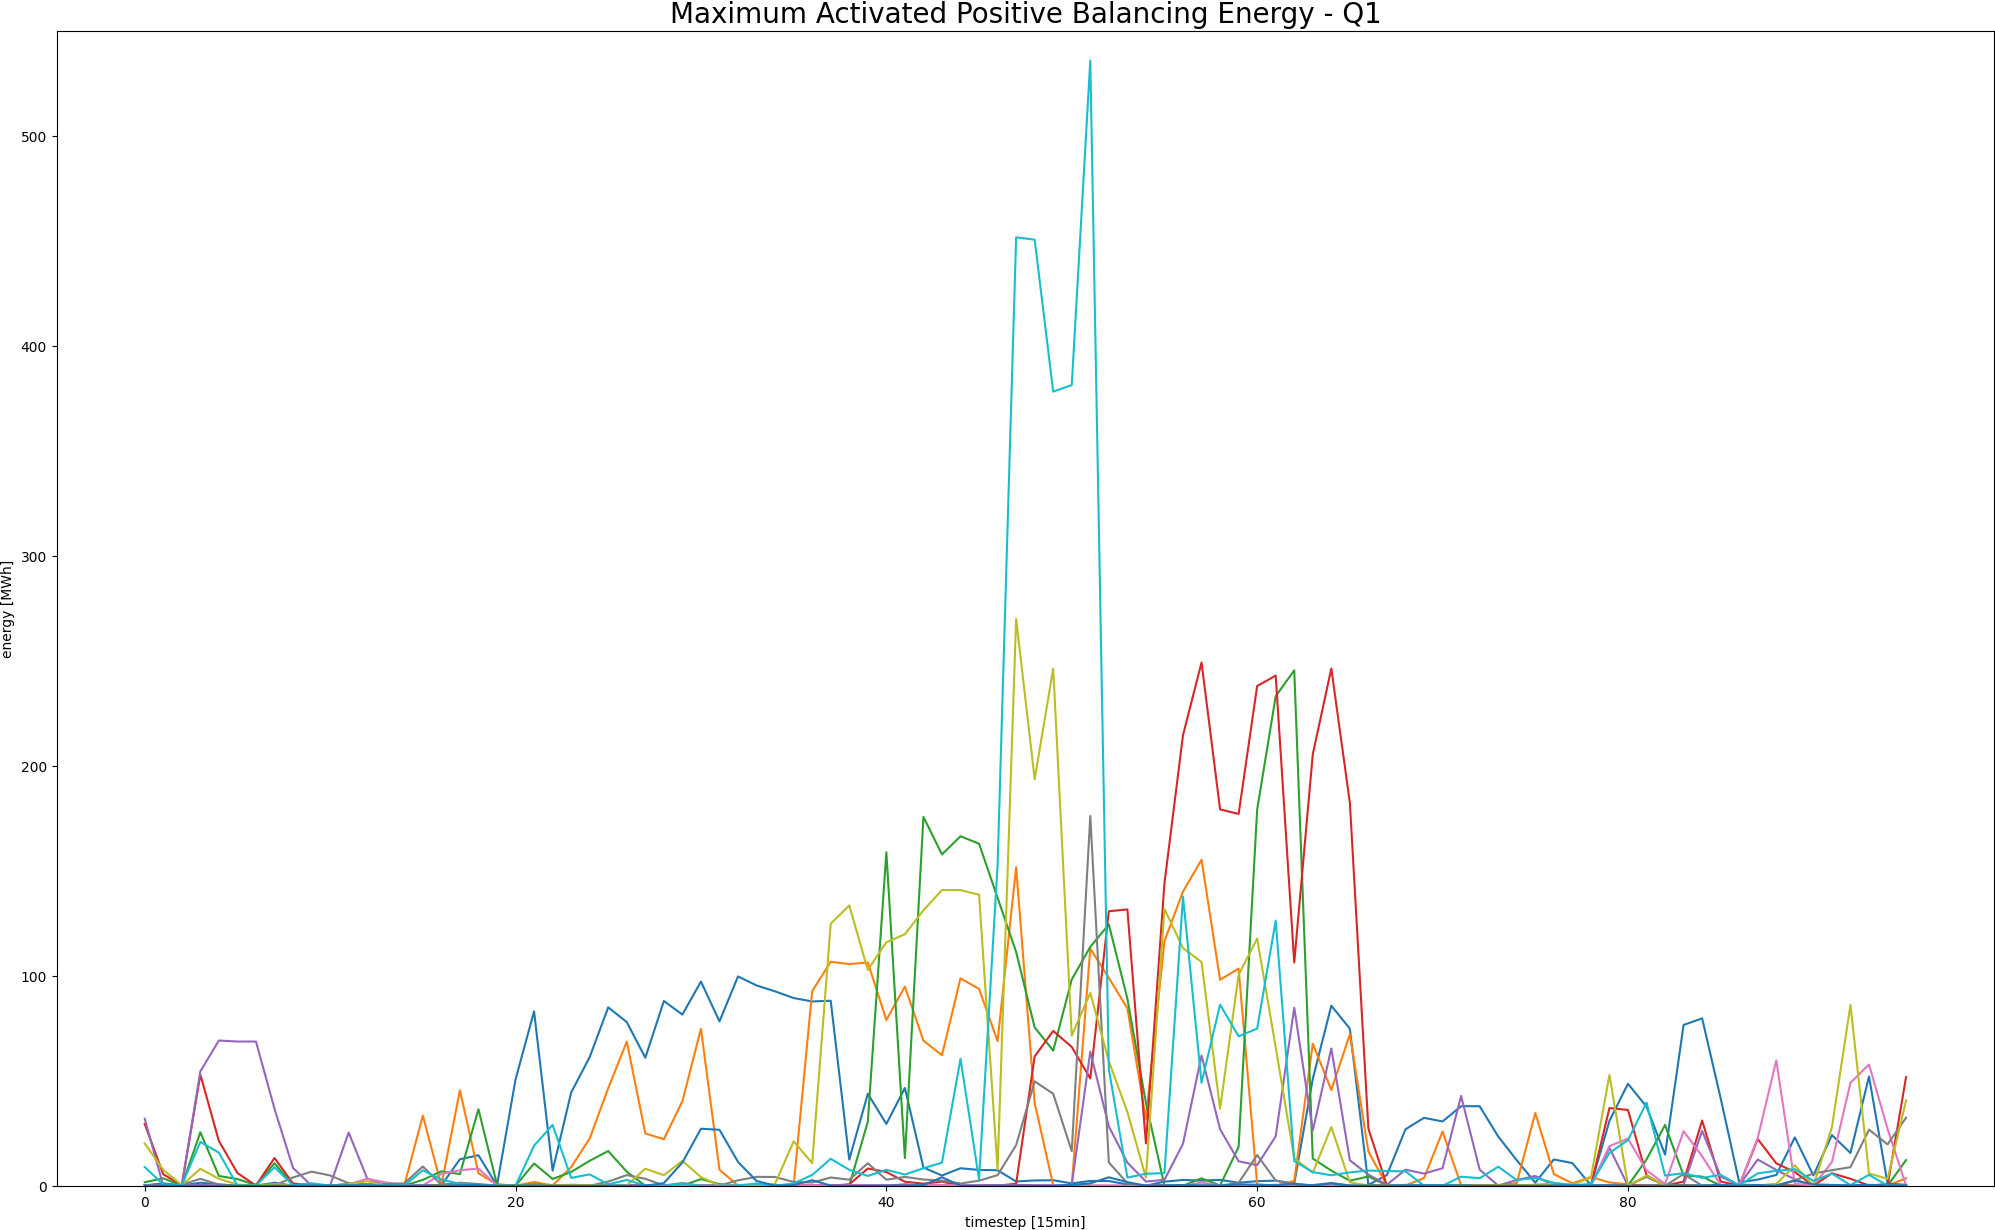
\includegraphics[width=1\linewidth]{pictures/results/Activated_posEnergy_Q1.png}
	\caption{Activated Positive Energy Q1}
	\label{fig:_posEnergy_Q1}
\end{figure}

\begin{figure}
	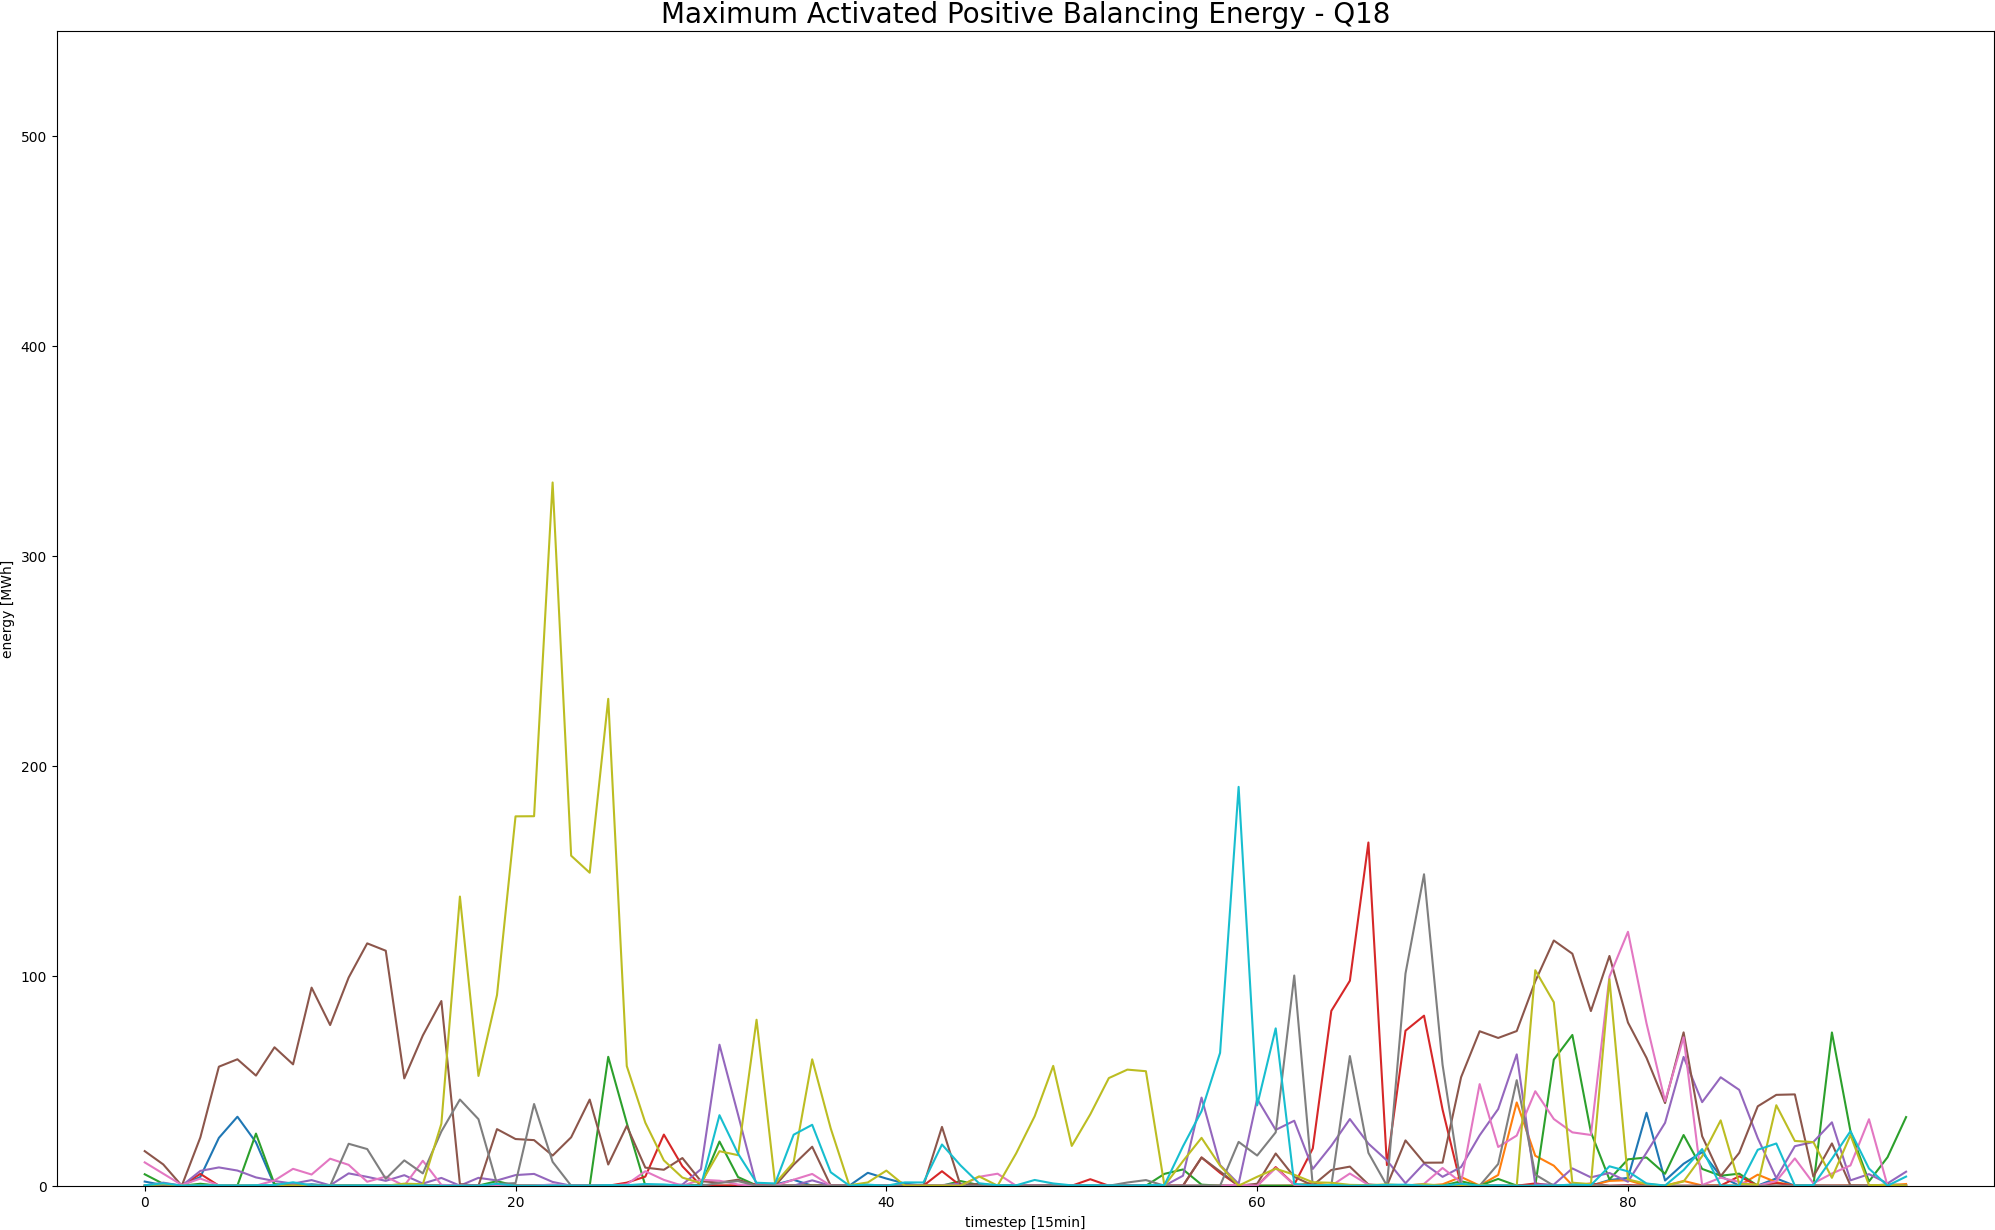
\includegraphics[width=1\linewidth]{pictures/results/Activated_posEnergy_Q18.png}
	\caption{Activated Positive Energy Q18}
	\label{fig:_posEnergy_Q18}
\end{figure}

\begin{figure}
	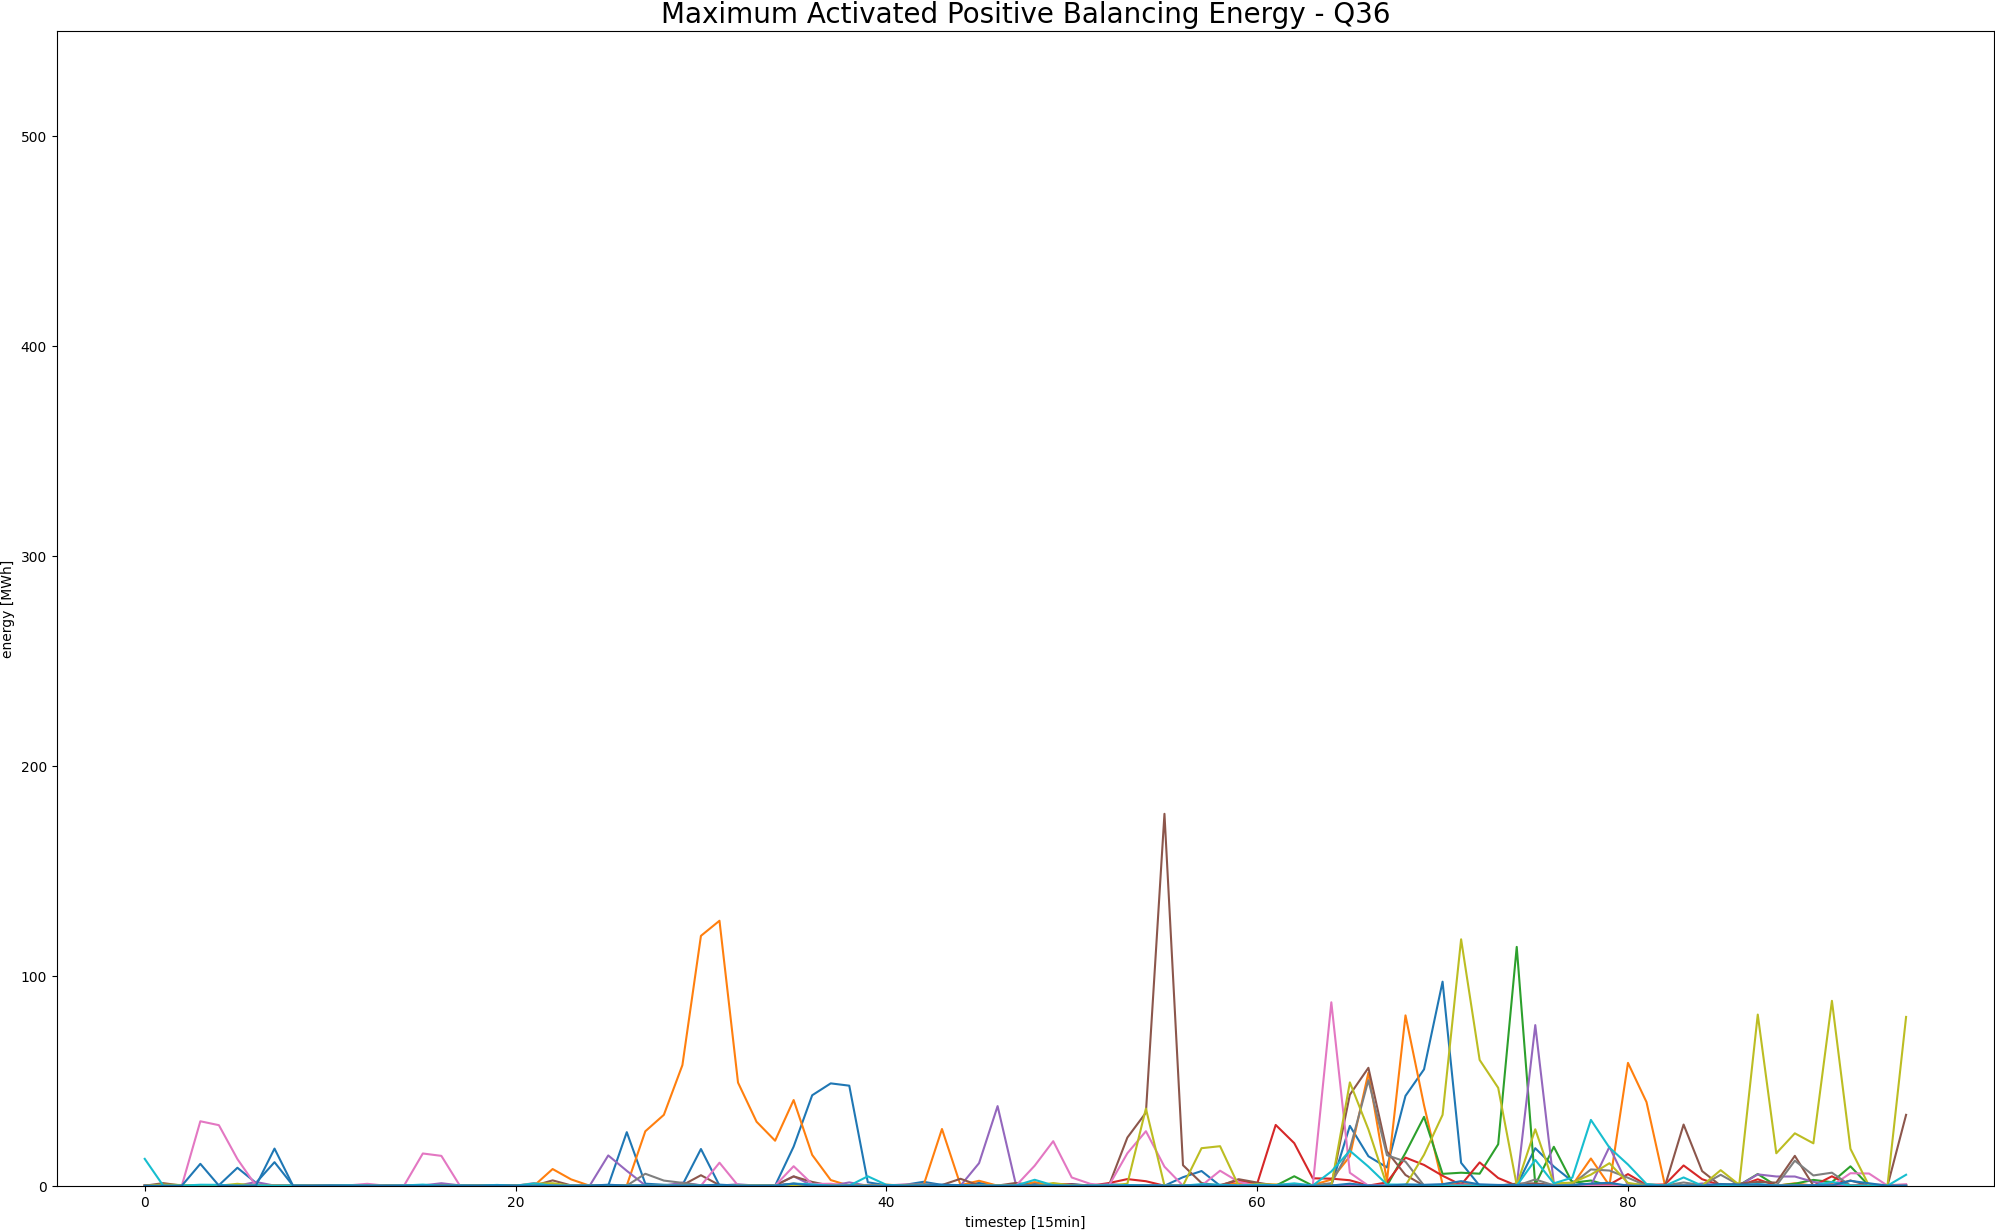
\includegraphics[width=1\linewidth]{pictures/results/Activated_posEnergy_Q36.png}
	\caption{Activated Positive Energy Q36}
	\label{fig:_posEnergy_Q36}
\end{figure}



\begin{figure}[H]
	\centering
	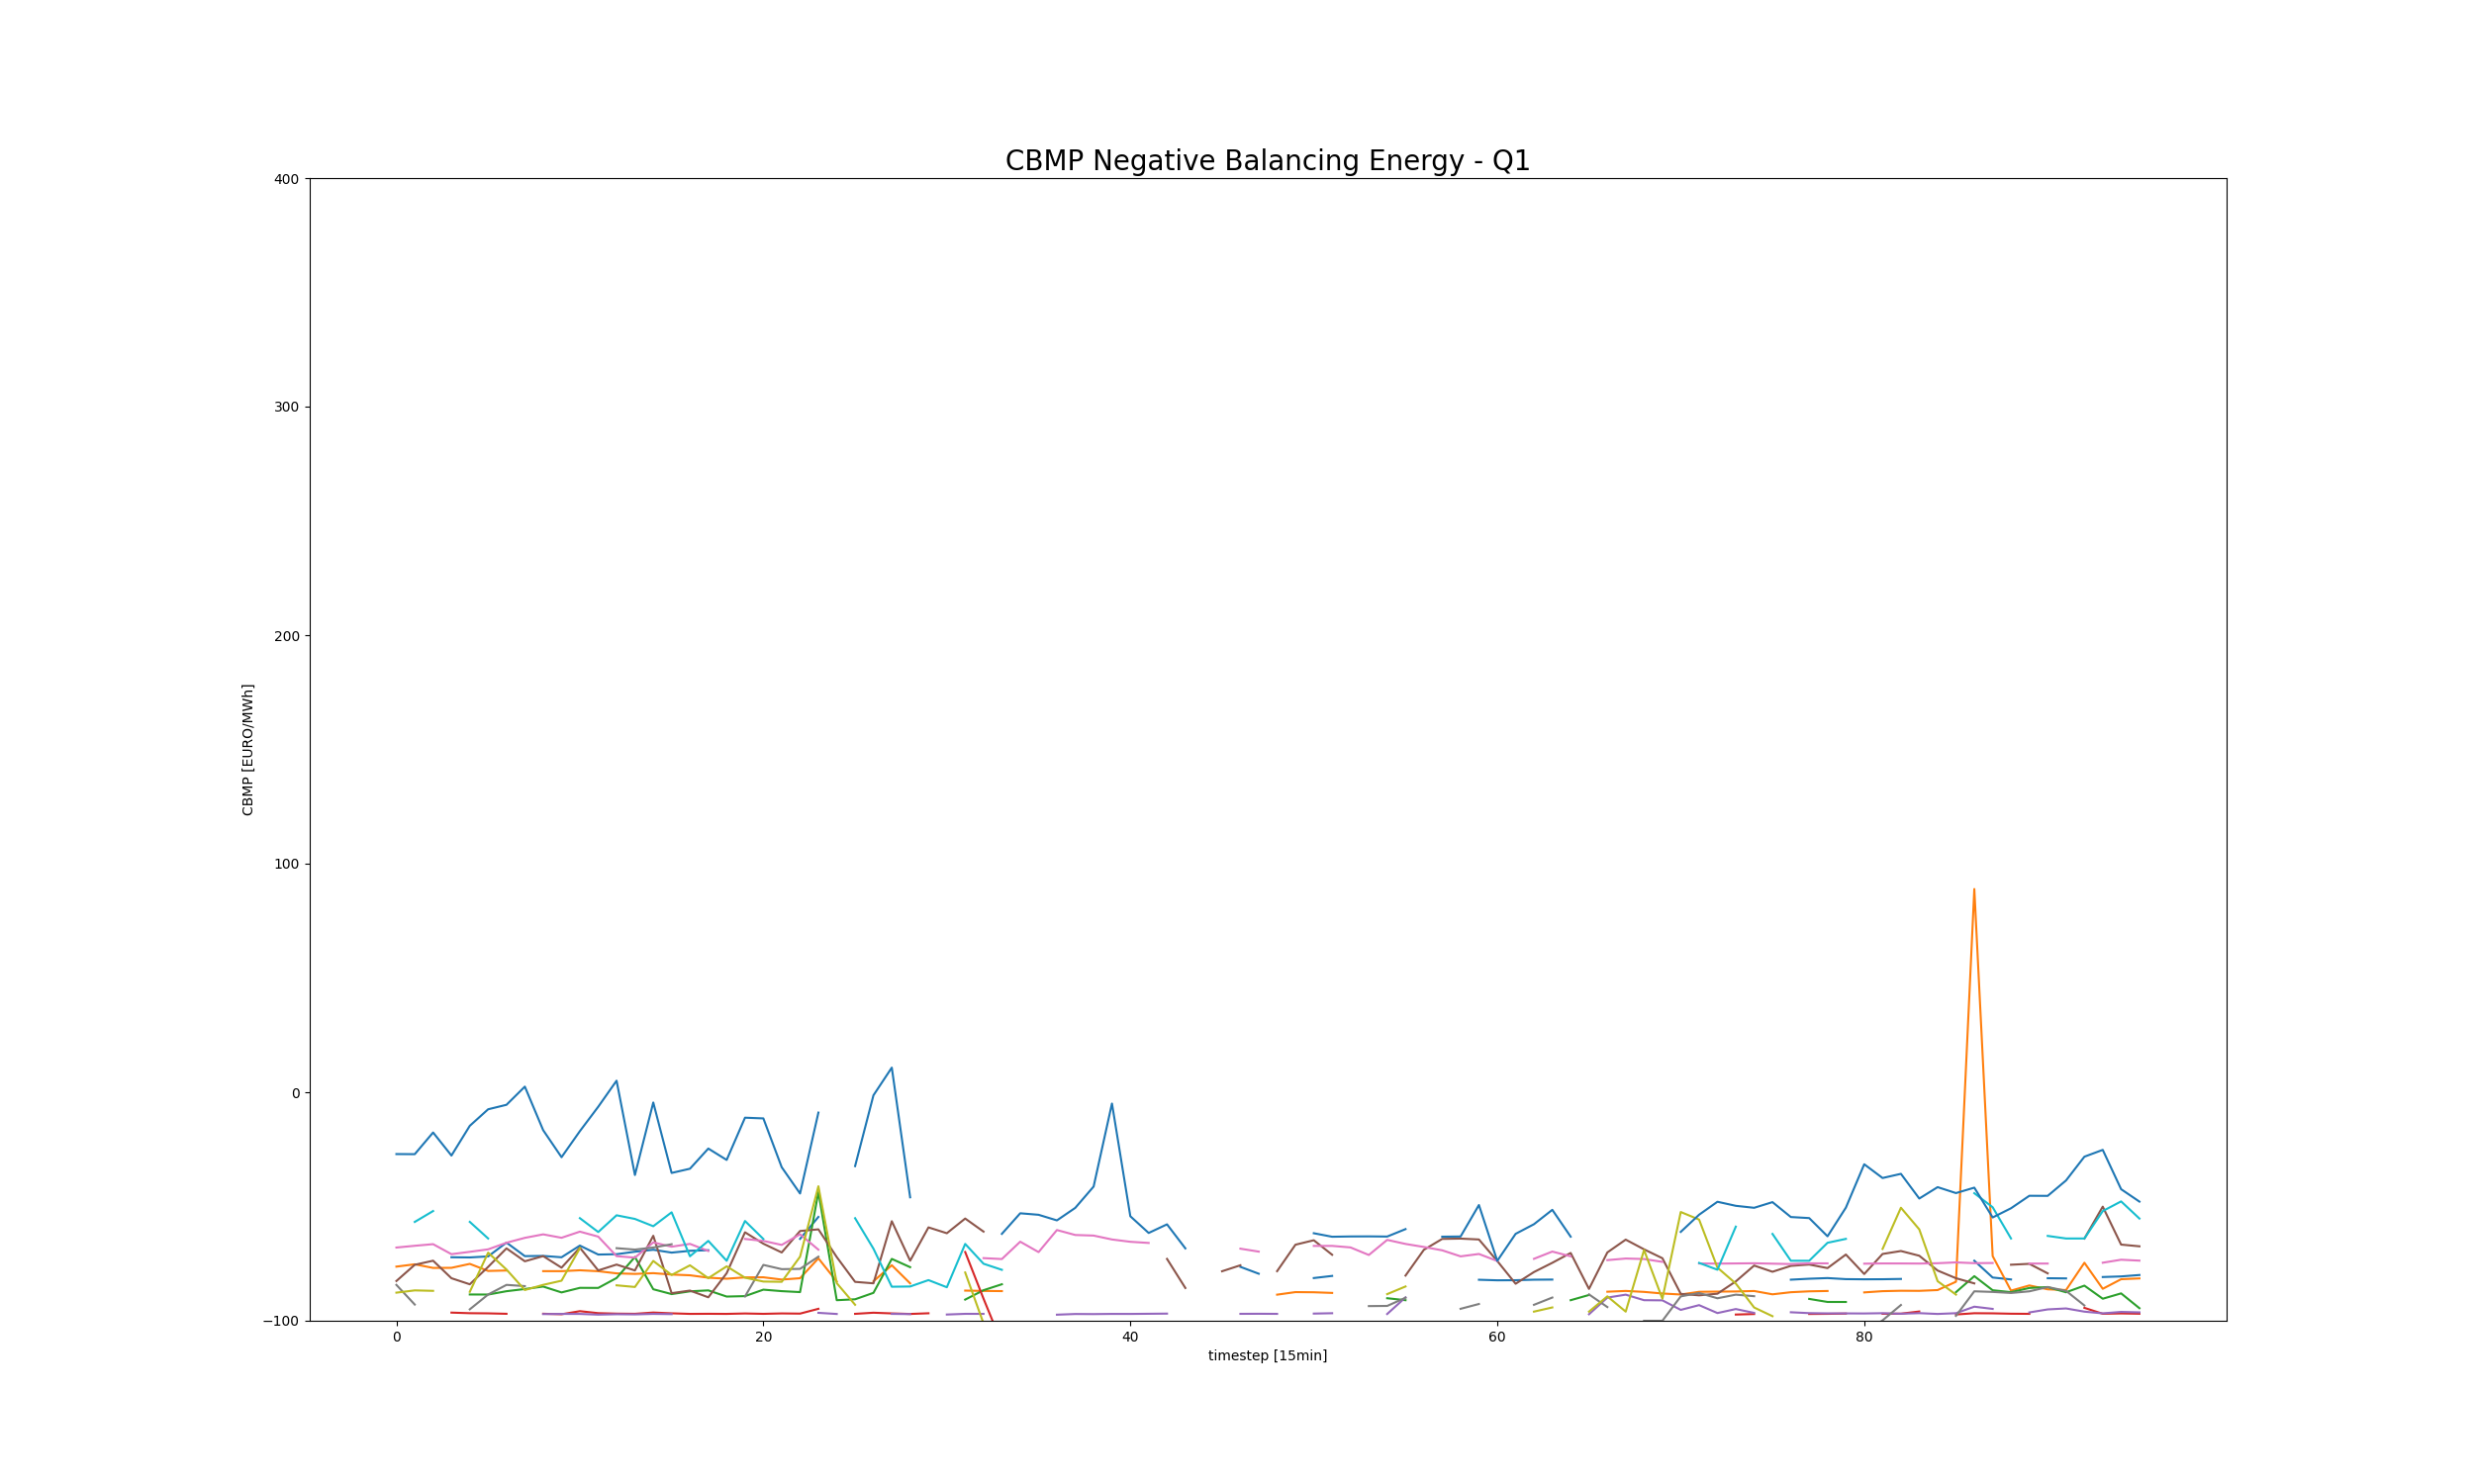
\includegraphics[width=1\linewidth]{pictures/results/CBMP_negBal_Q1.png}
	\caption{CBMP Negative Energy Q1}
	\label{fig:CBMP_negBal_Q1}
\end{figure}


\begin{figure}[H]
	\centering
	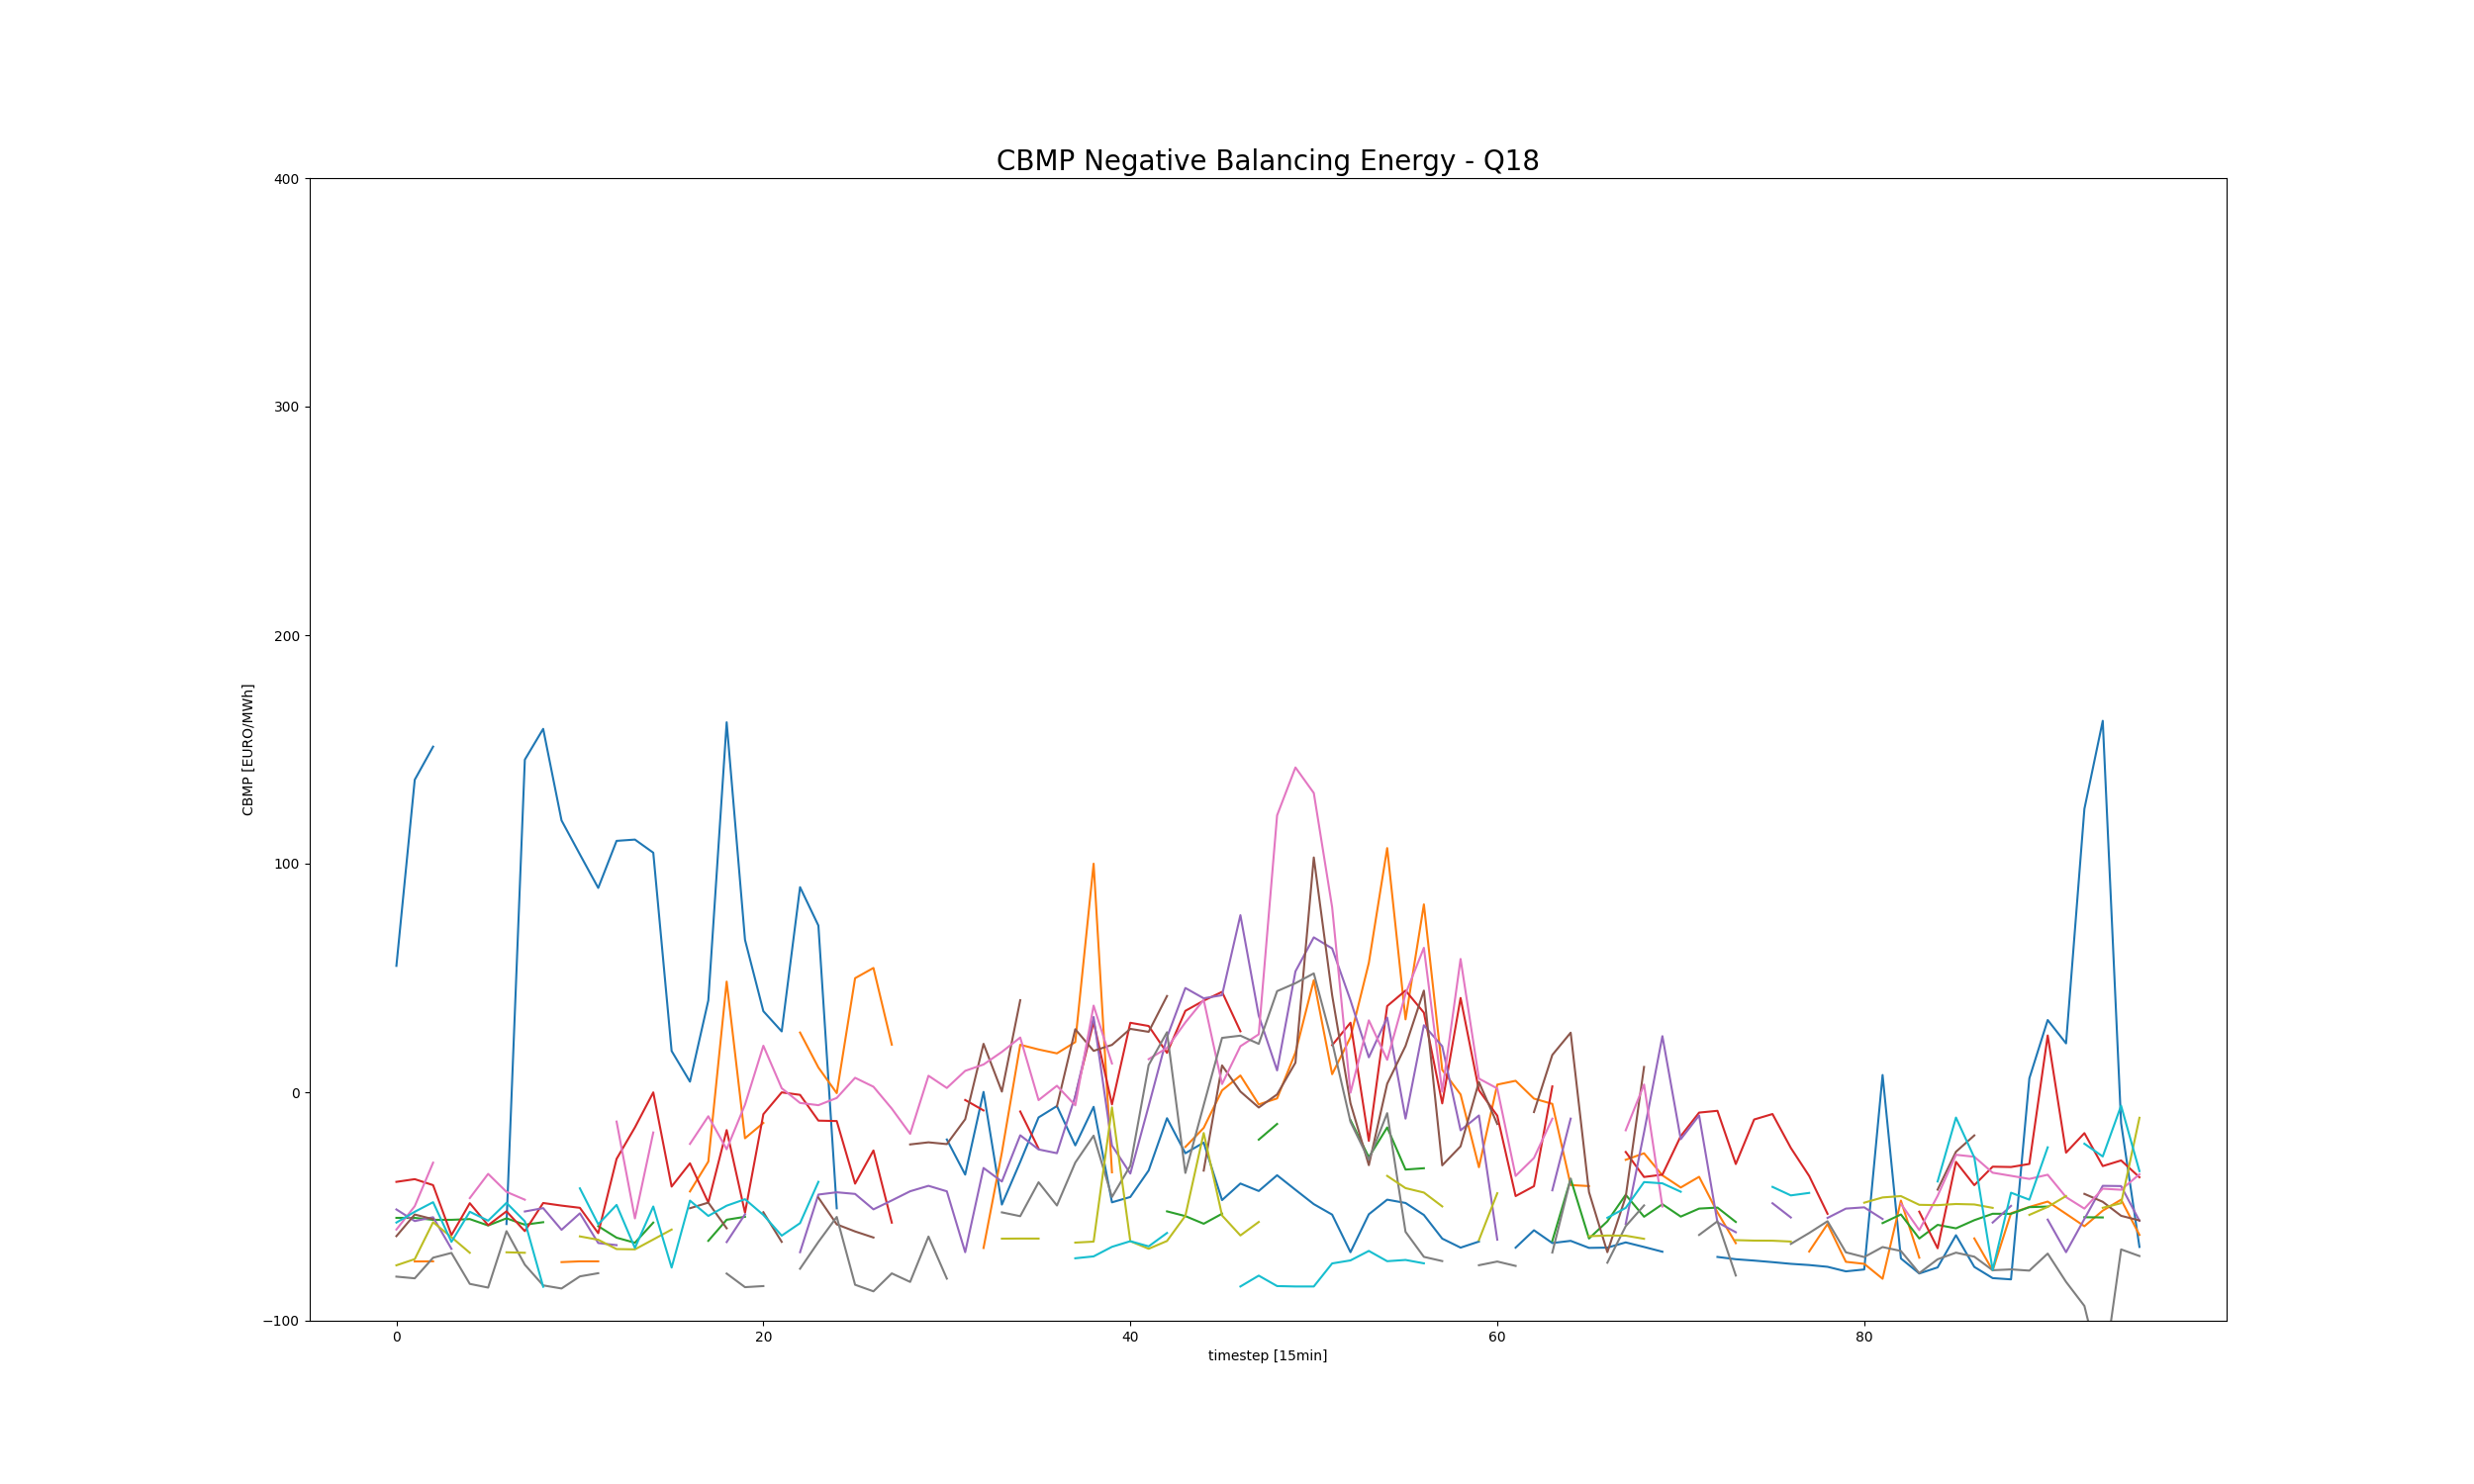
\includegraphics[width=1\linewidth]{pictures/results/CBMP_negBal_Q18.png}
	\caption{CBMP Negative Energy Q18}
	\label{fig:CBMP_negBal_Q18}
\end{figure}


\begin{figure}[H]
	\centering
	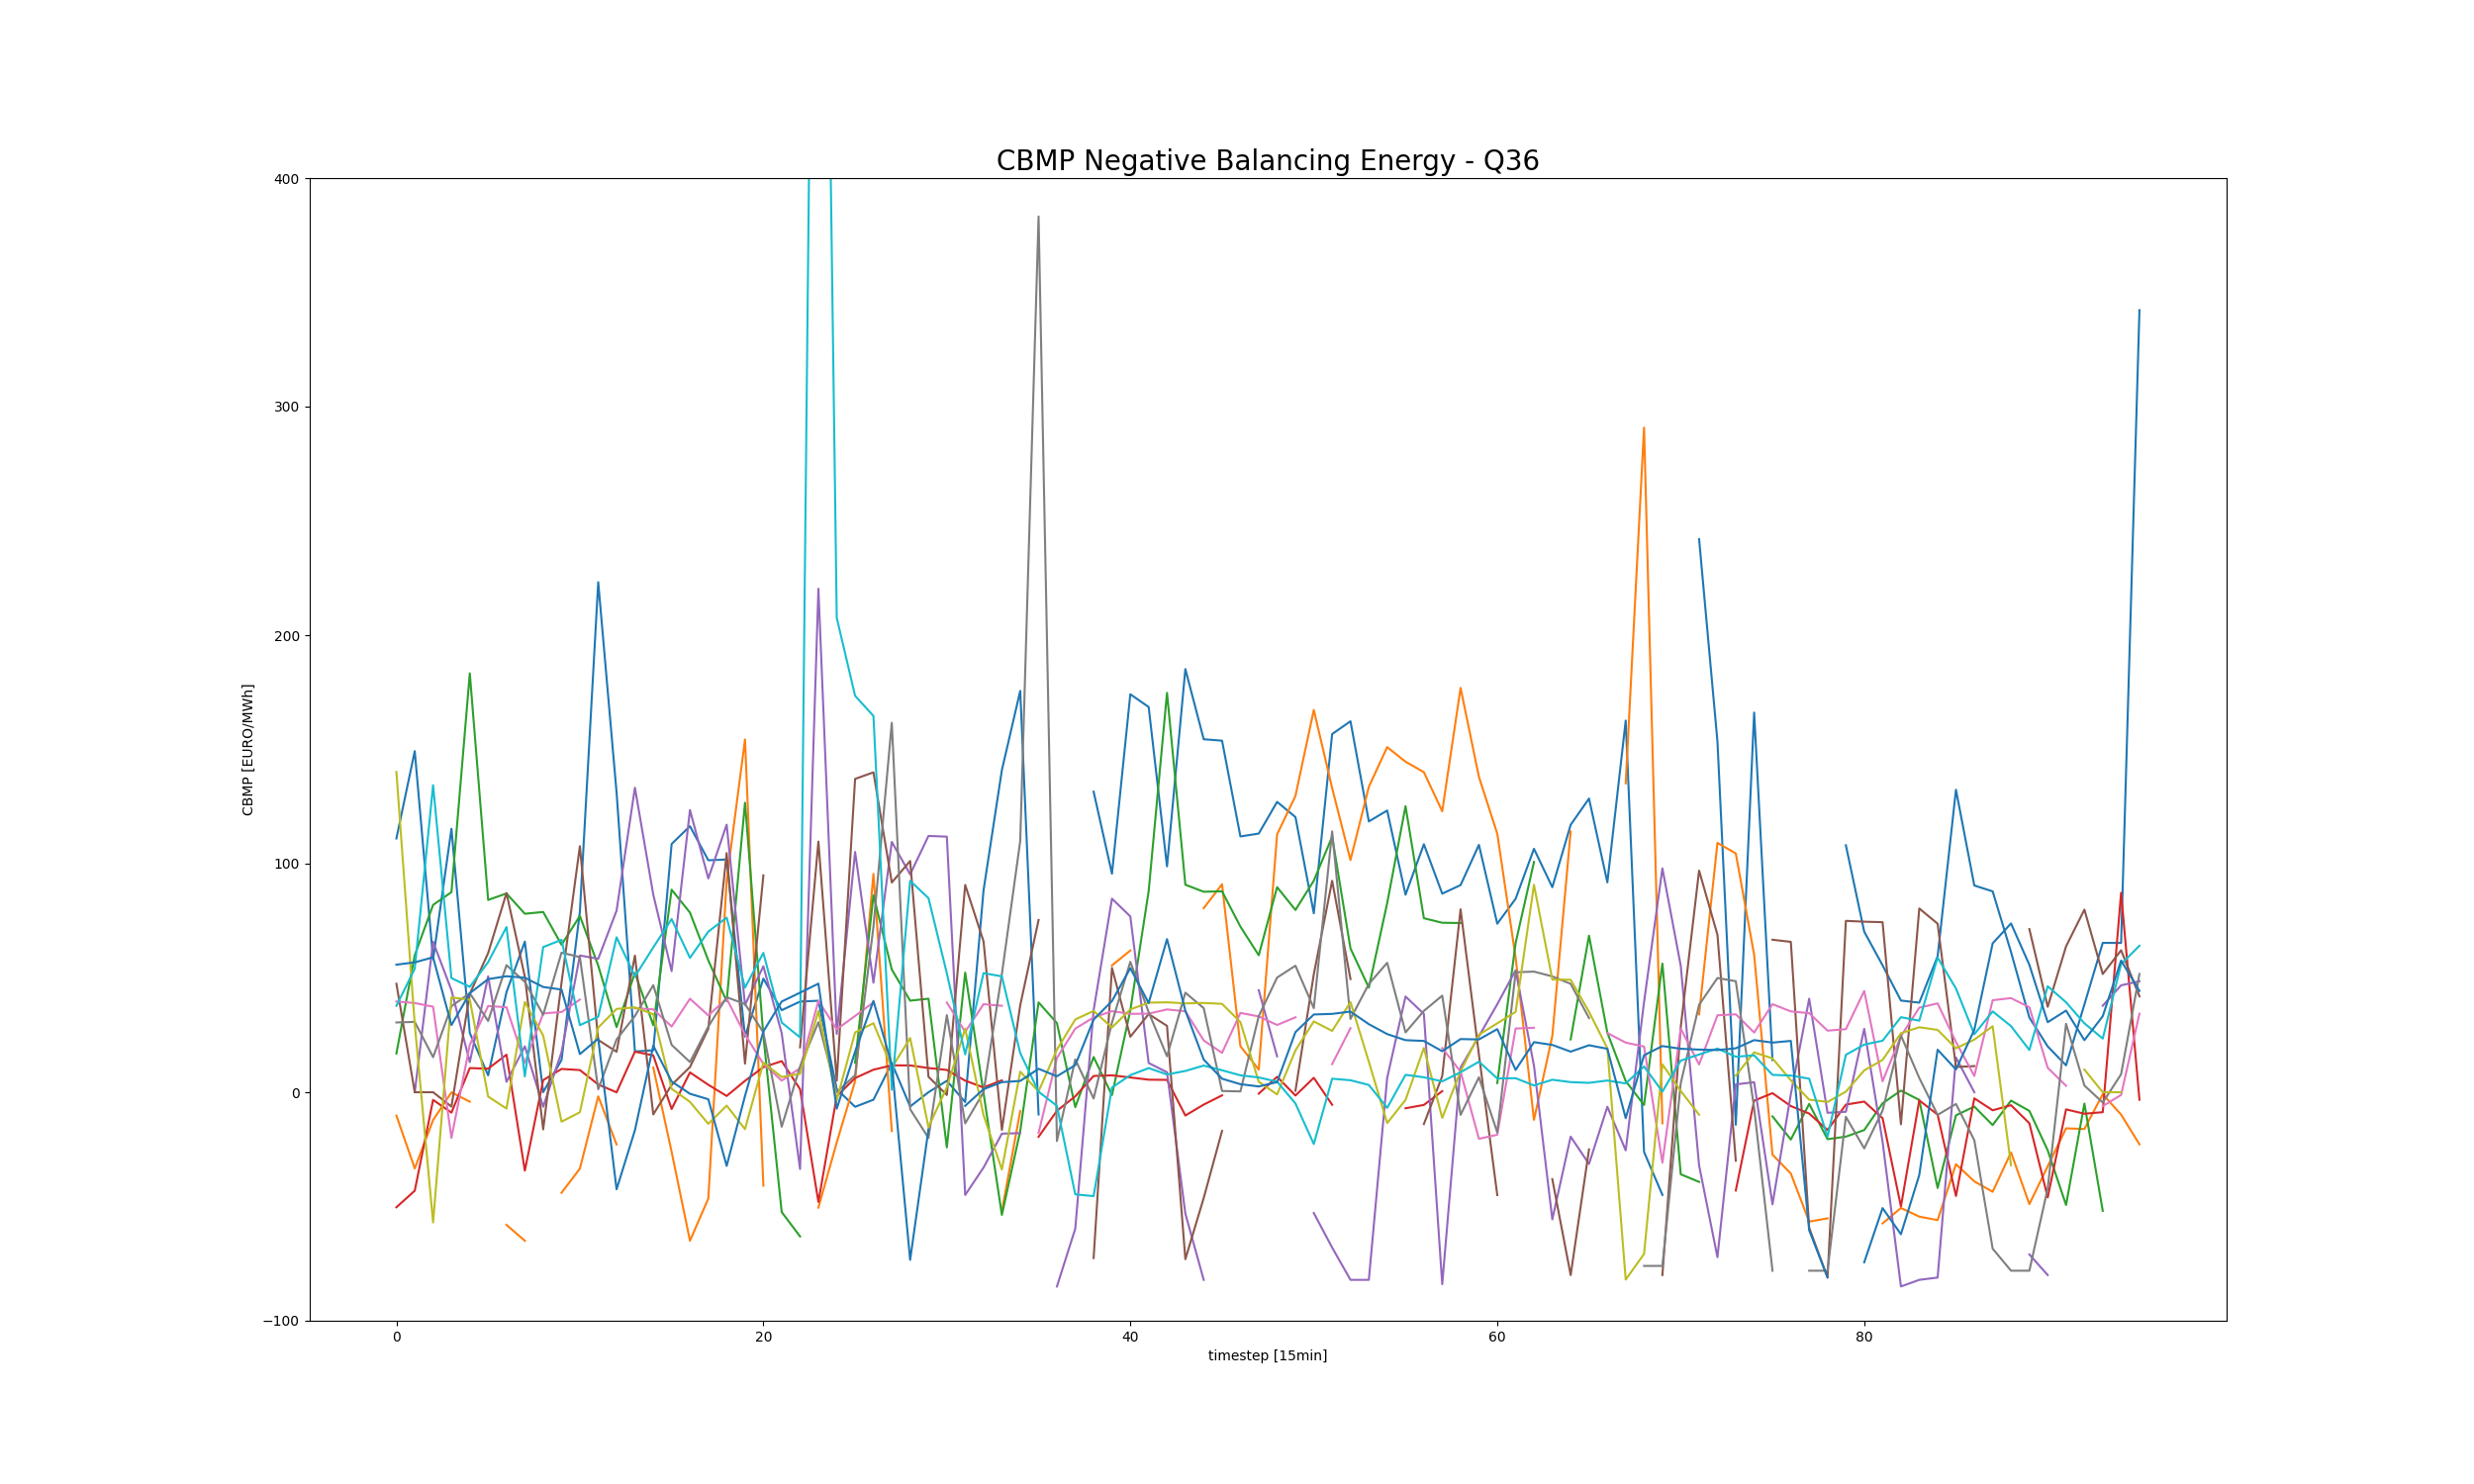
\includegraphics[width=1\linewidth]{pictures/results/CBMP_negBal_Q36.png}
	\caption{CBMP Negative Energy Q36}
	\label{fig:CBMP_negBal_Q36}
\end{figure}

\begin{figure}
	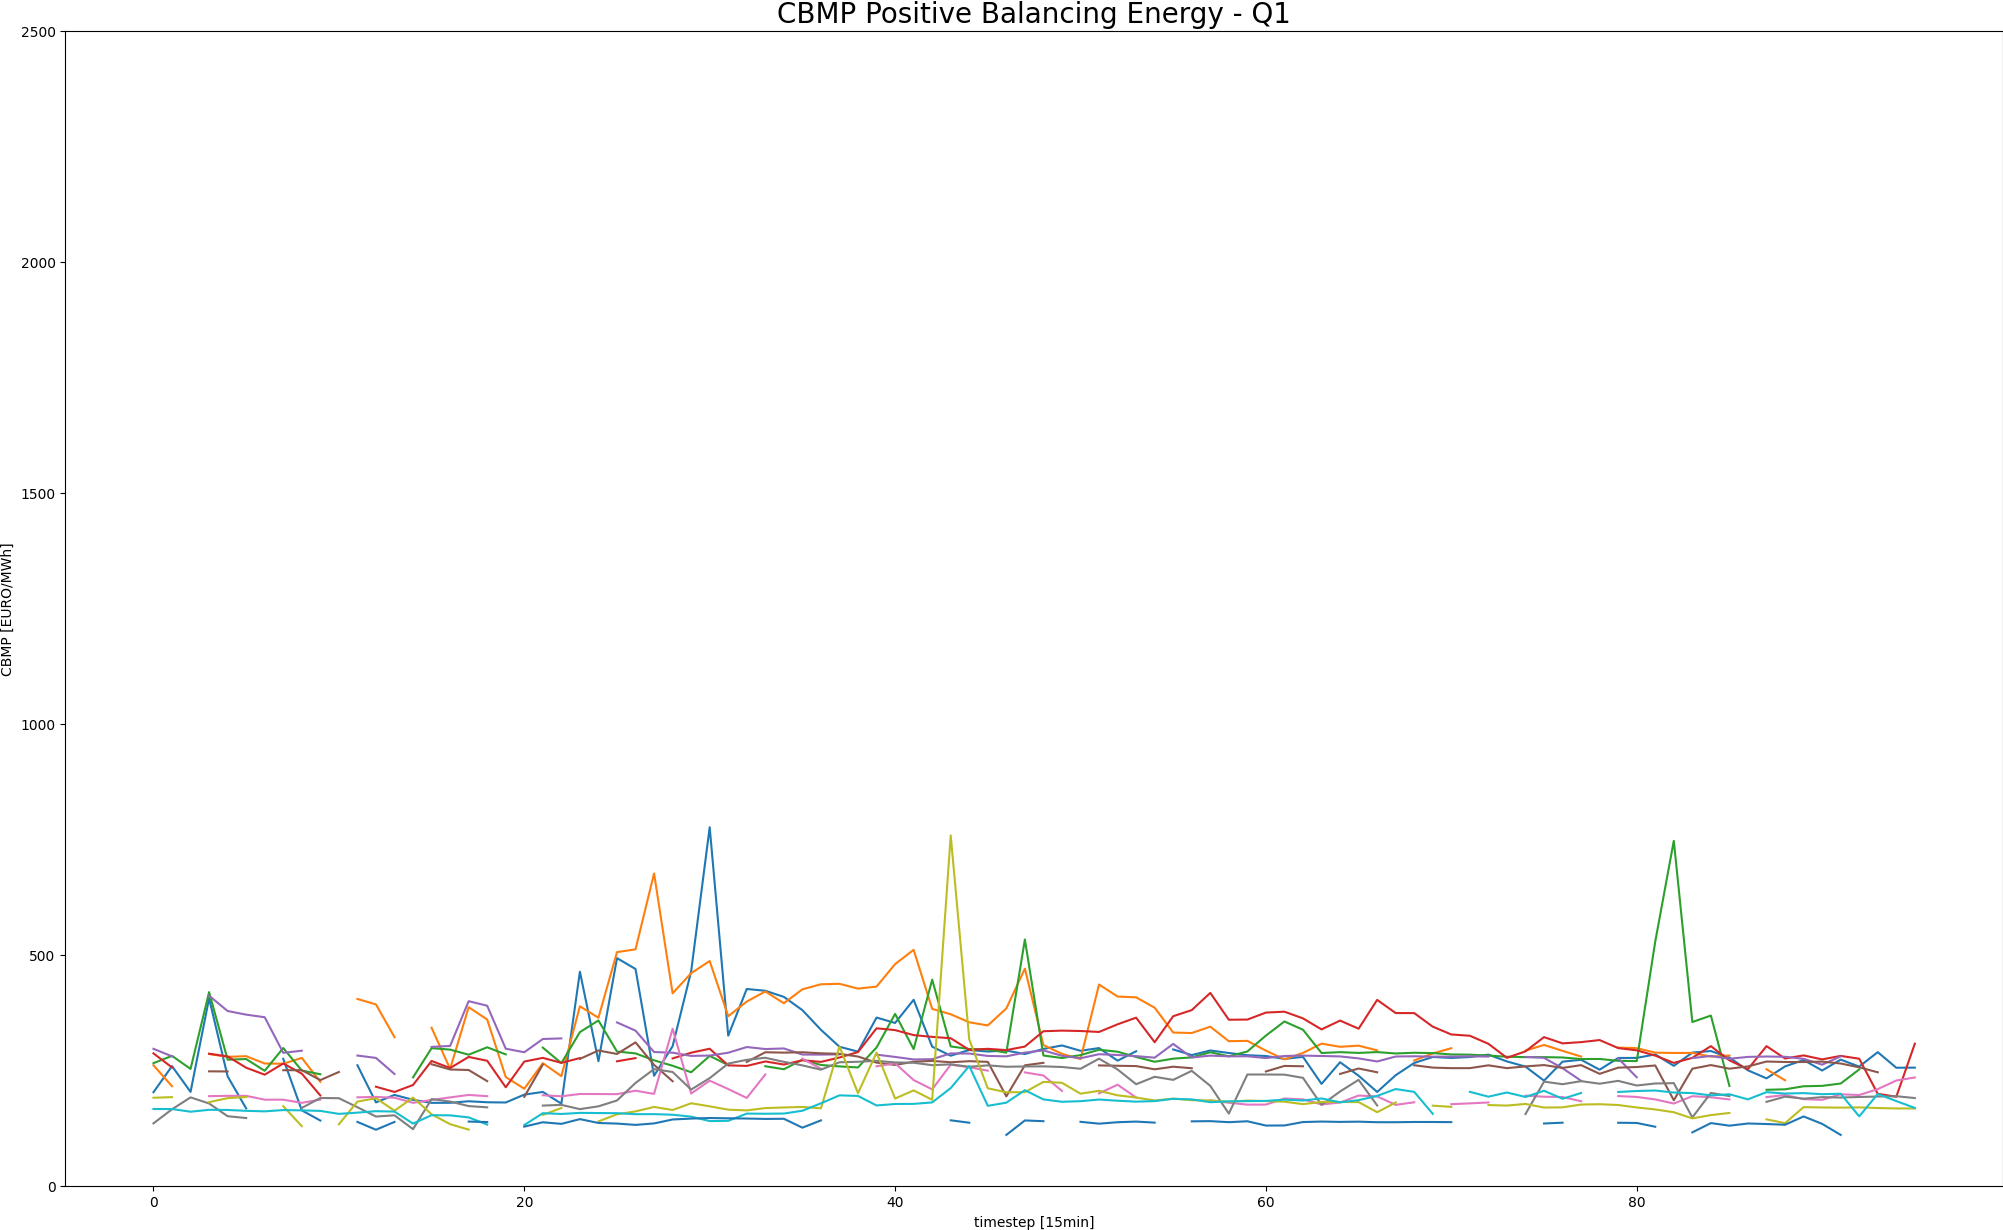
\includegraphics[width=1\linewidth]{pictures/results/CBMP_PosBal_Q1.png}
	\caption{CBMP Positive Energy Q1}
	\label{fig:CBMP_PosBal_Q1}
\end{figure}

\begin{figure}
	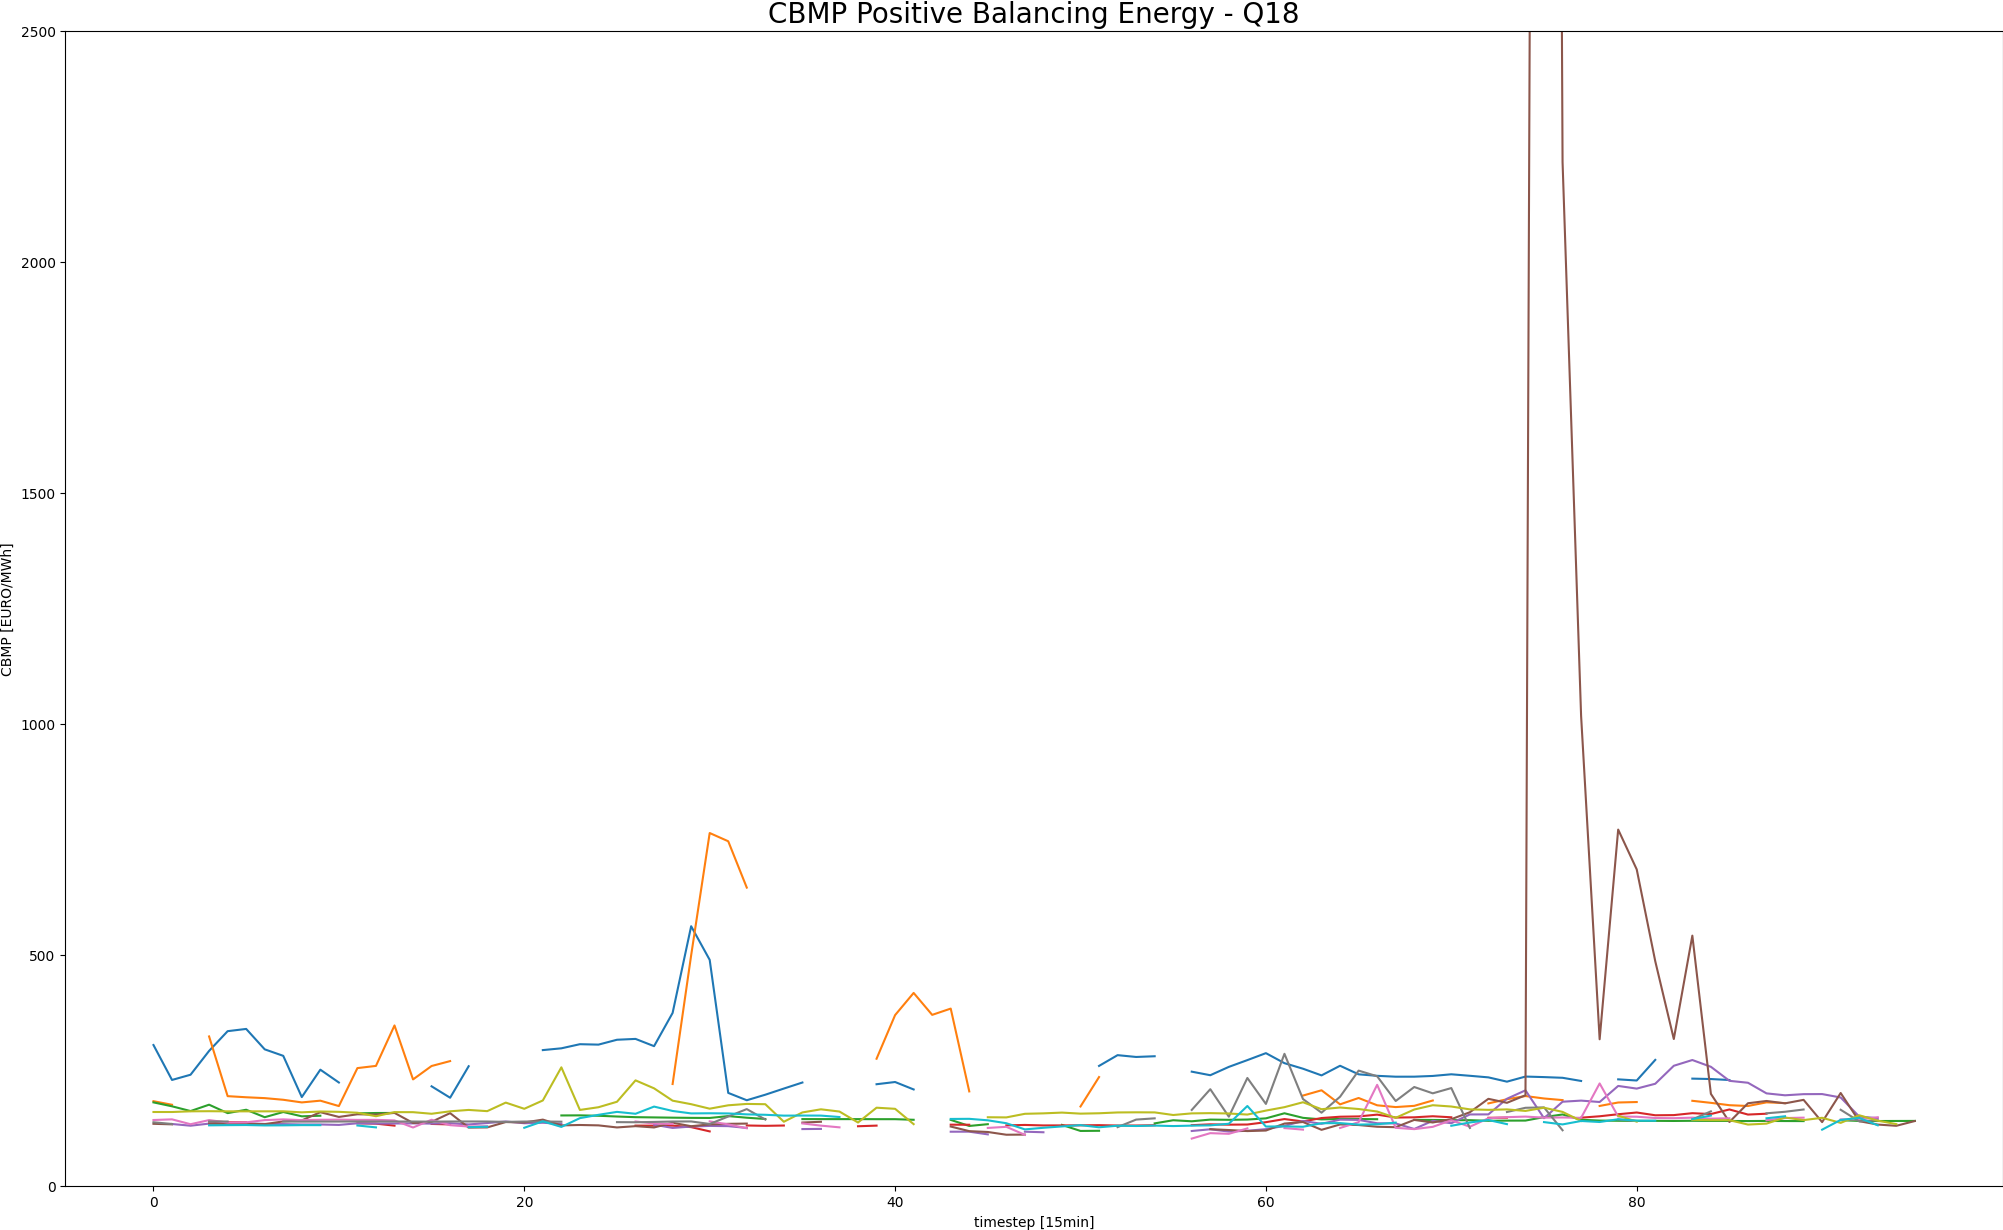
\includegraphics[width=1\linewidth]{pictures/results/CBMP_PosBal_Q18.png}
	\caption{CBMP Positive Energy Q18}
	\label{fig:CBMP_PosBal_Q18}
\end{figure}
\begin{figure}
	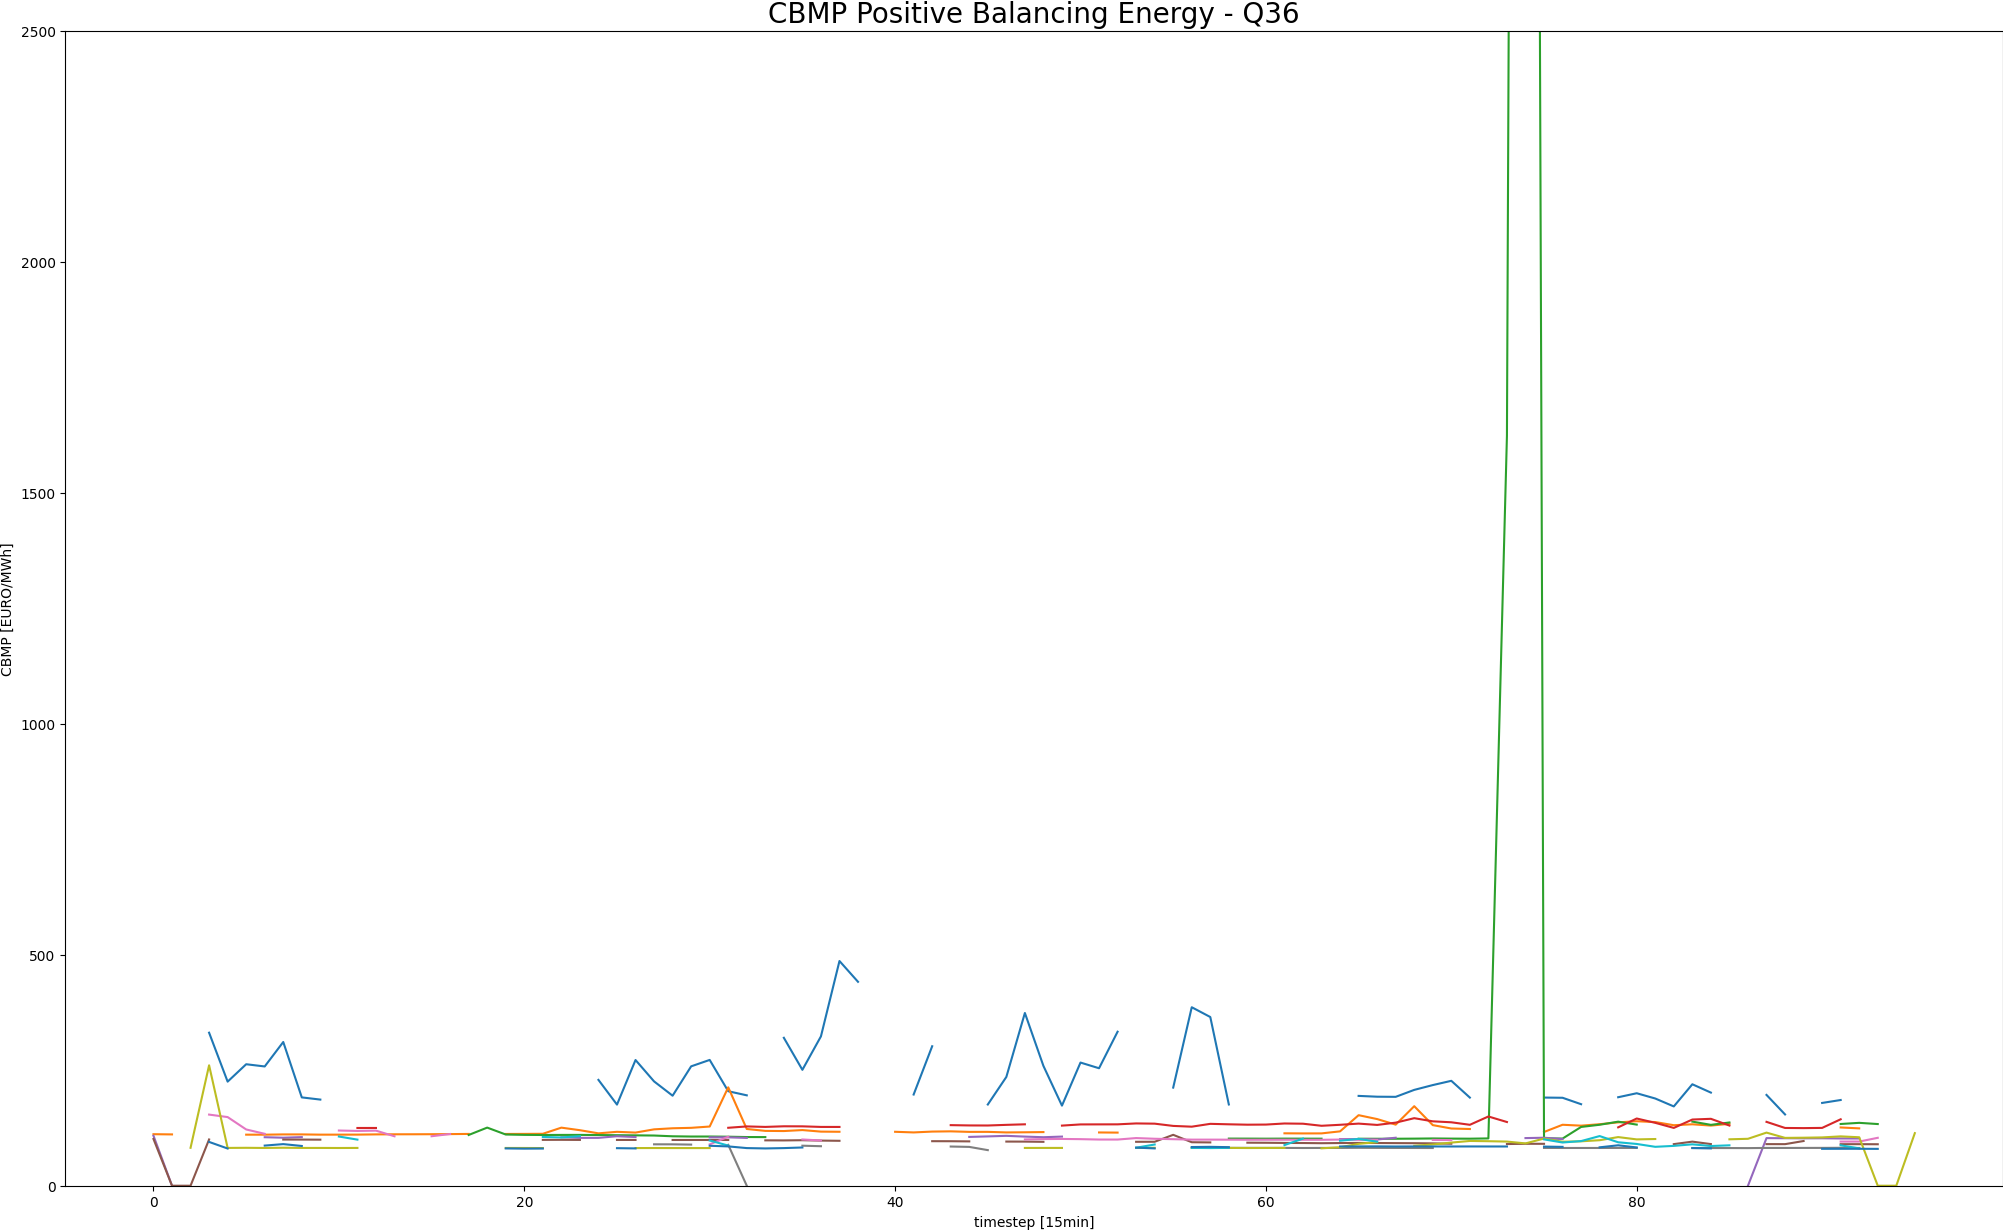
\includegraphics[width=1\linewidth]{pictures/results/CBMP_PosBal_Q36.png}
	\caption{CBMP Positive Energy Q36}
	\label{fig:CBMP_PosBal_Q36}
\end{figure}

Für den selben Zeitabschnitt lässt sich der DA Markt wie folgt zusammenfassen:
\begin{figure}[H]
	\centering
	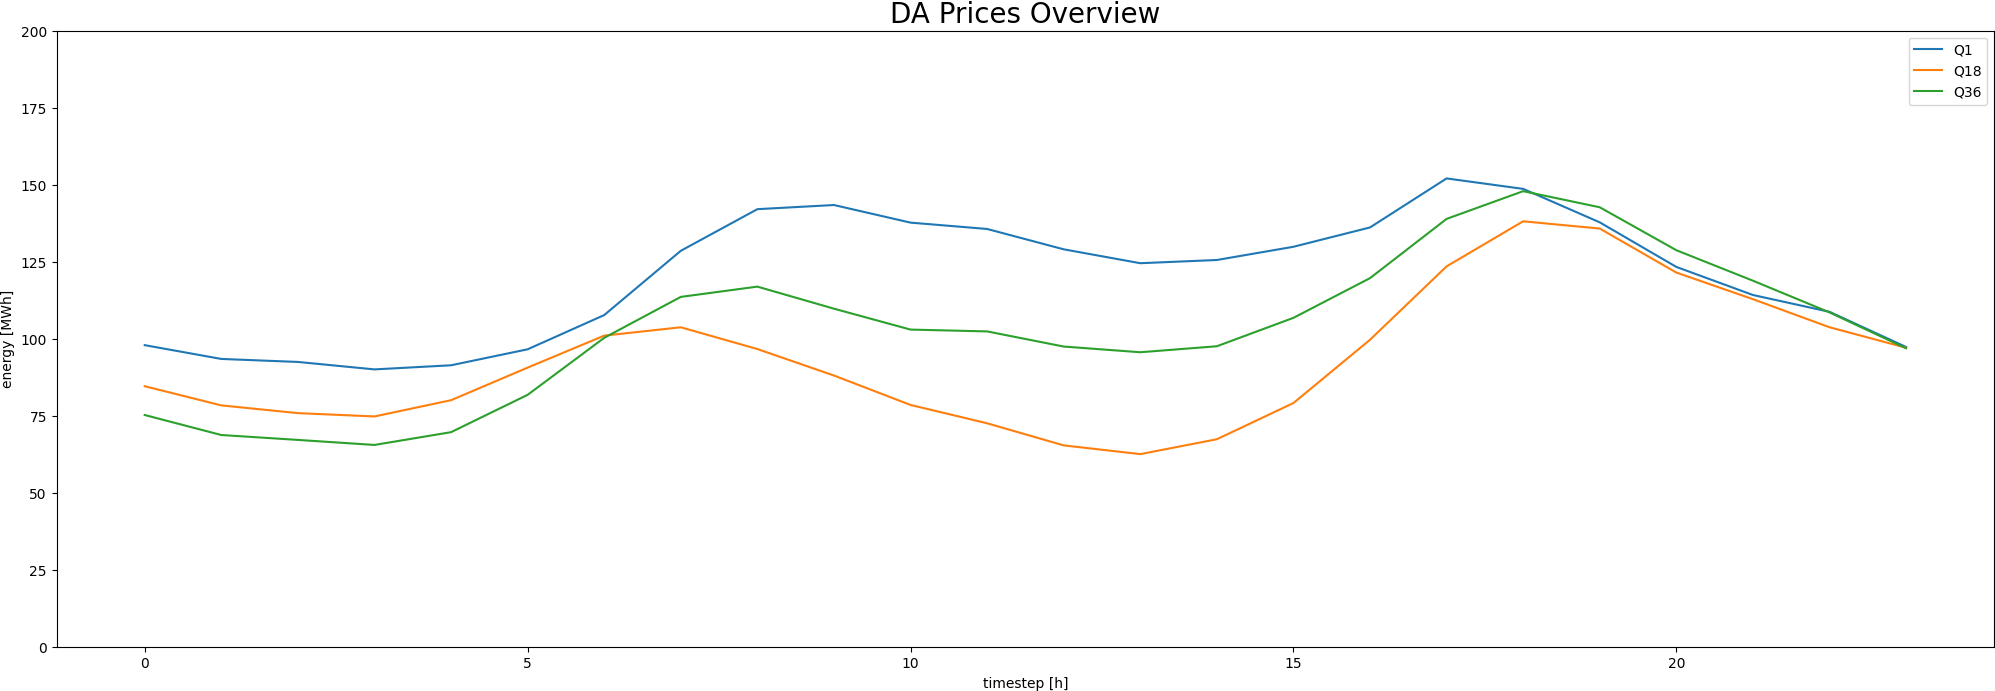
\includegraphics[width=1\linewidth]{pictures/results/DAPrices.png}
	\caption{DA Prices}
	\label{fig:DAPrices}
\end{figure}
\begin{figure}
	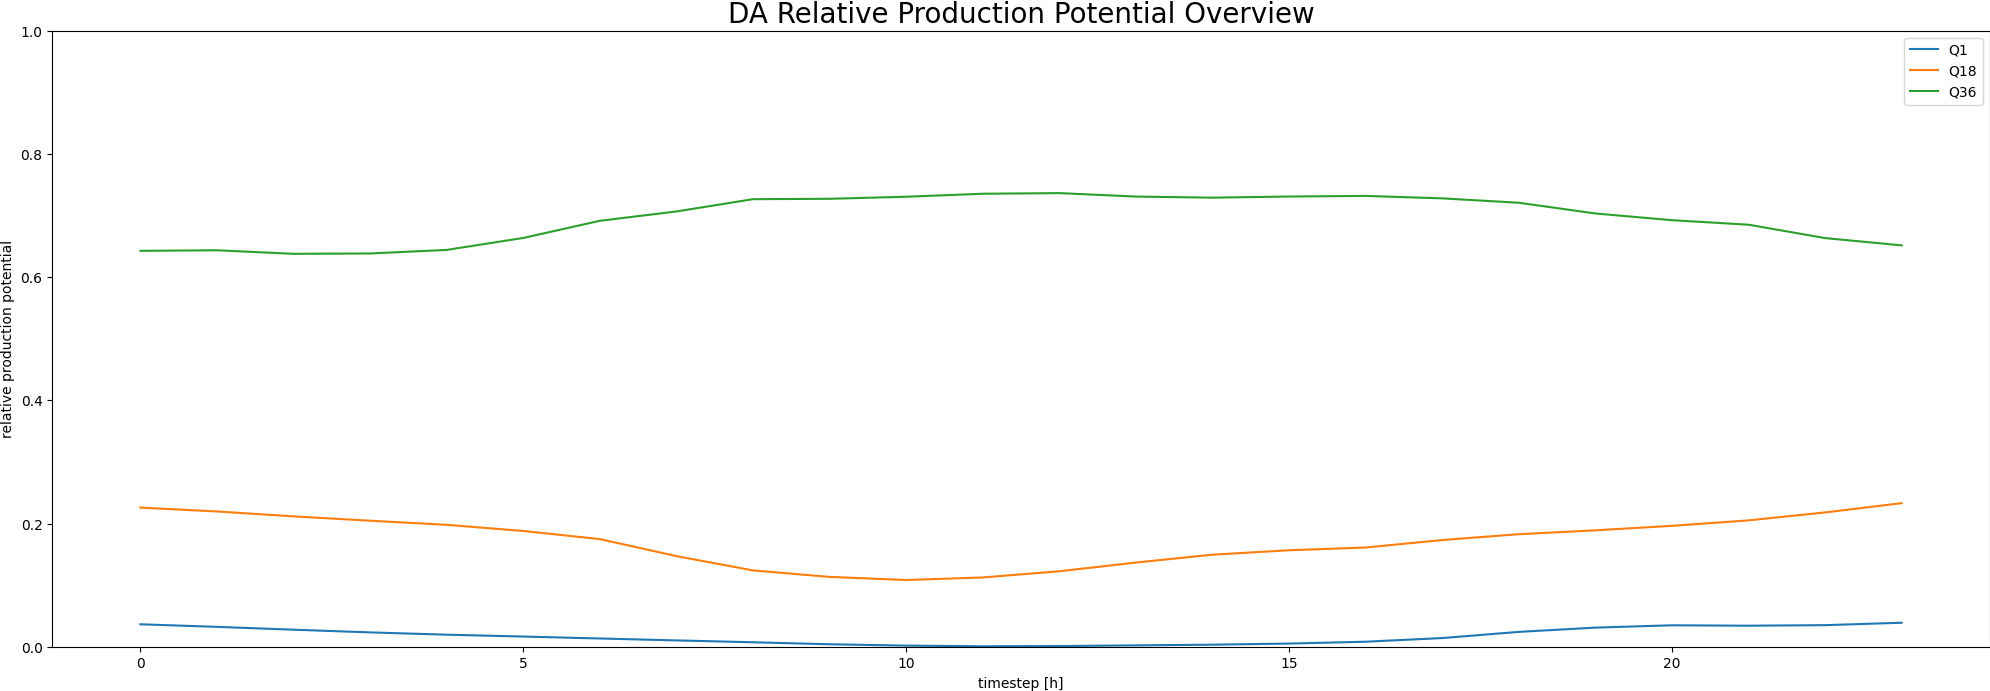
\includegraphics[width=1\linewidth]{pictures/results/DAProd.png}
	\caption{DA Production}
	\label{fig:DAProd}
\end{figure}

Außerdem stellt sich der entsprechende RL Markt wie folgt dar:

\begin{figure}[H]
	\centering
	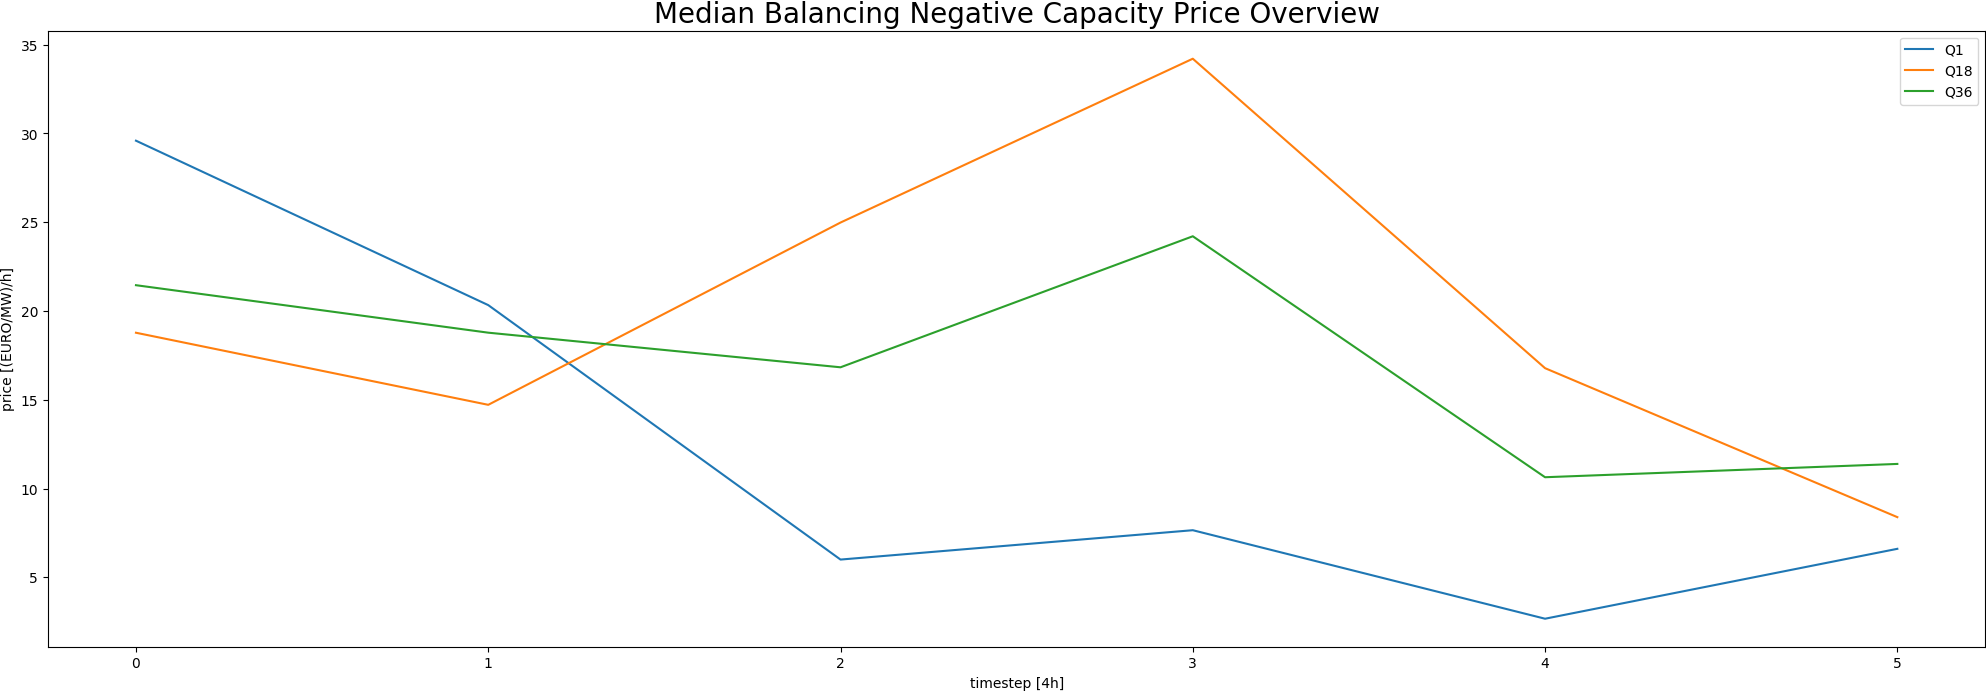
\includegraphics[width=1\linewidth]{pictures/results/RL_negPrice_Overview.png}
	\caption{RL Negative Prices}
	\label{fig:RL_negPrice_Overview}
\end{figure}
\begin{figure}
	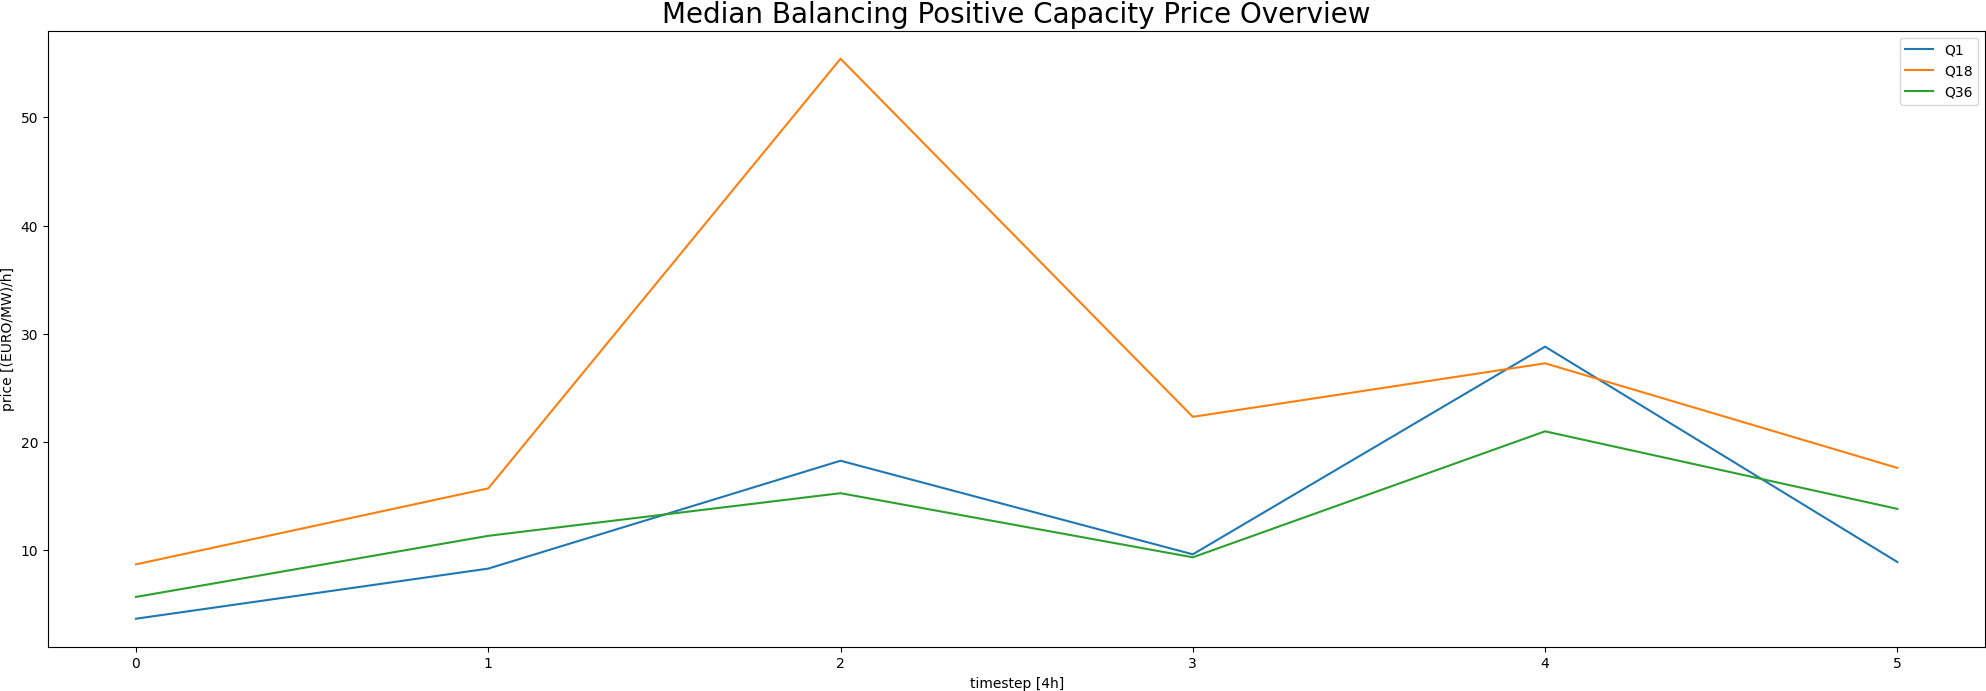
\includegraphics[width=1\linewidth]{pictures/results/RL_posPrice_Overview.png}
	\caption{RL Negative Prices}
	\label{fig:RL_posPrice_Overview}
\end{figure}

\section{Model Results}

\begin{figure}[H]
	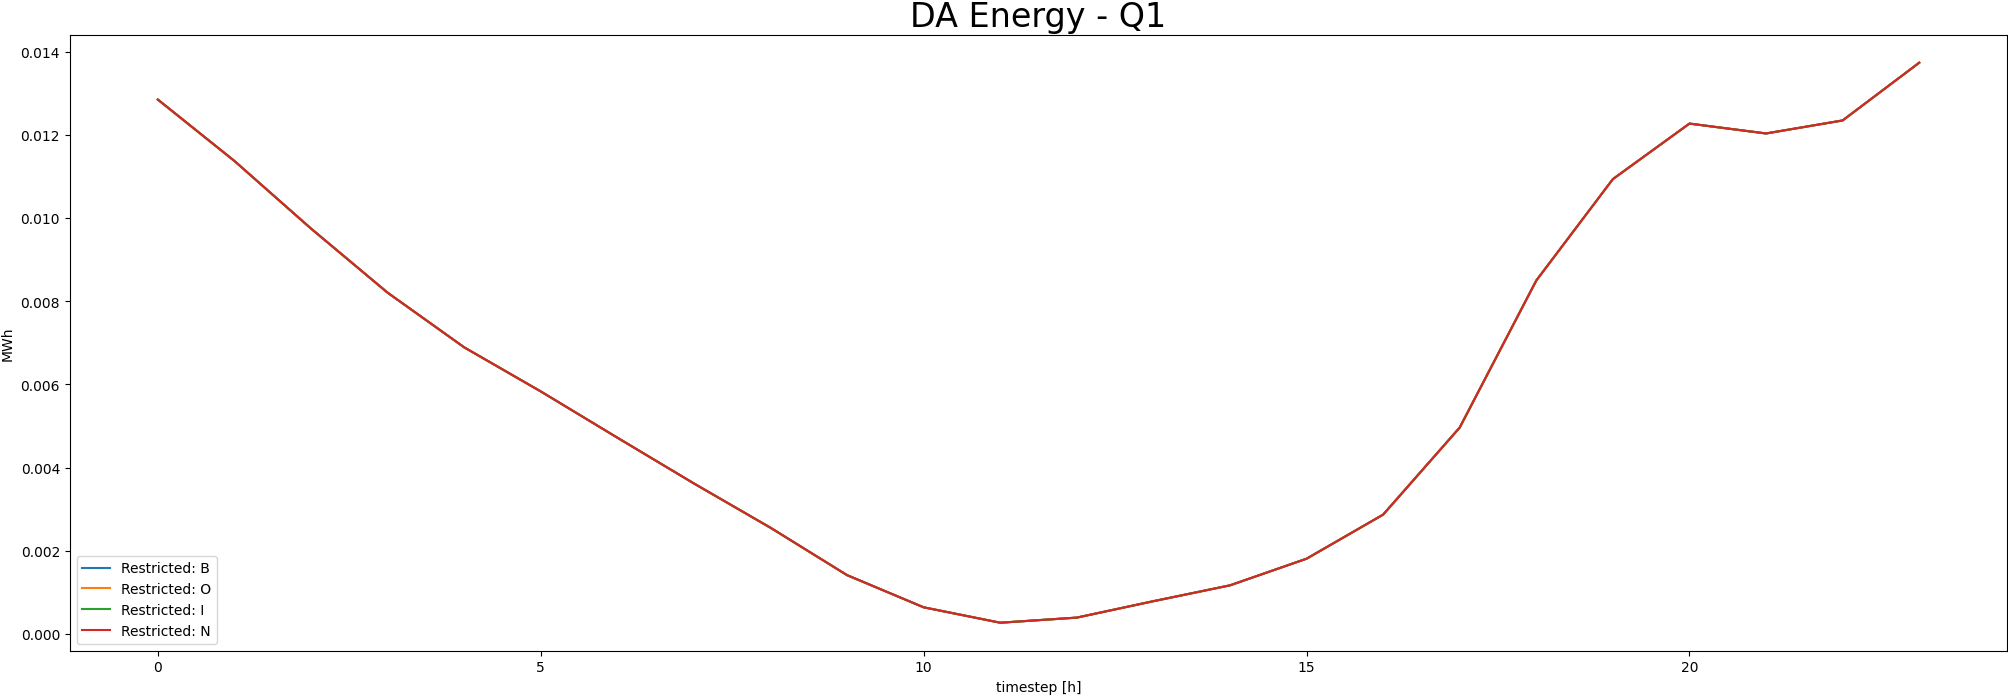
\includegraphics[width=1\linewidth]{pictures/results/DA Energy - Q1.png}
	\caption{DA Energy - Q1}
	\label{fig:DA Energy - Q1}
\end{figure}

\begin{figure}[H]
	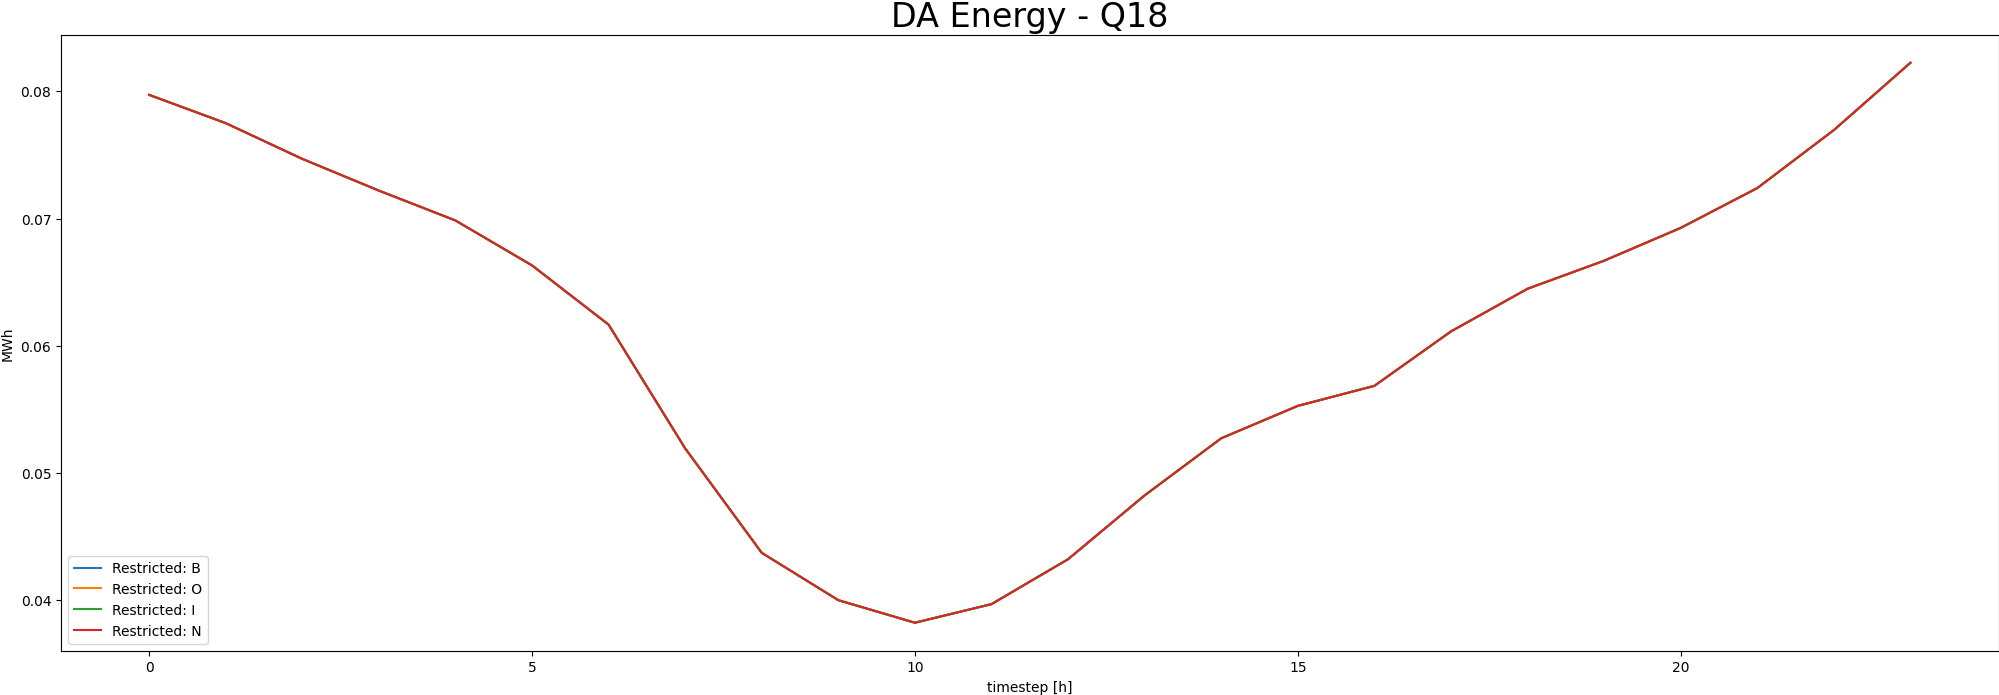
\includegraphics[width=1\linewidth]{pictures/results/DA Energy - Q18.png}
	\caption{DA Energy - Q18}
	\label{fig:DA Energy - Q18}
\end{figure}

\begin{figure}[H]
	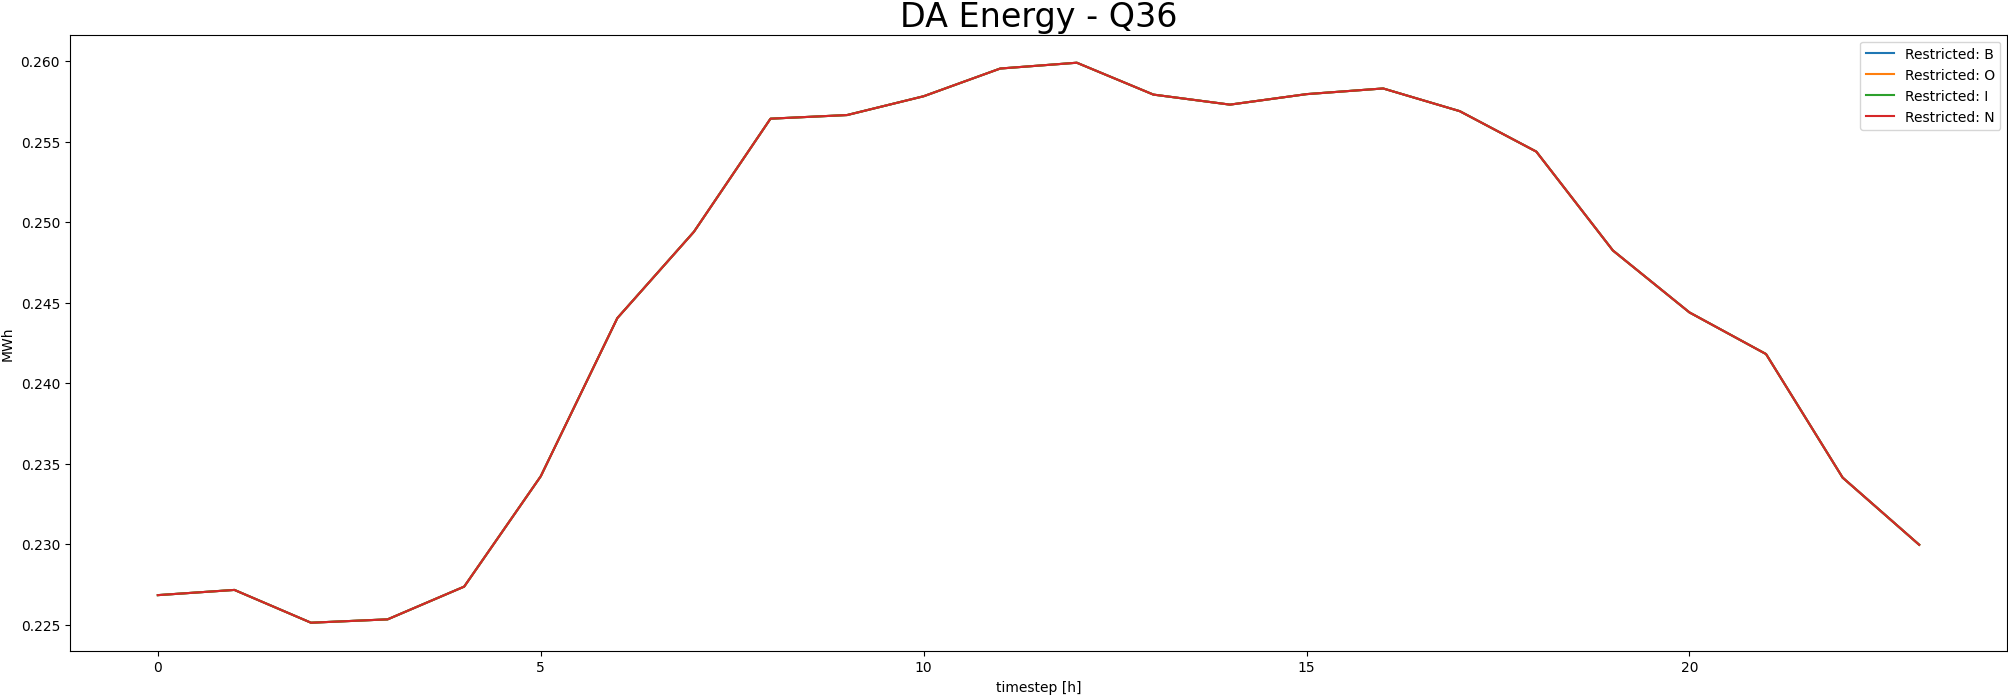
\includegraphics[width=1\linewidth]{pictures/results/DA Energy - Q36.png}
	\caption{DA Energy - Q36}
	\label{fig:DA Energy - Q36}
\end{figure}
\begin{figure}[H]
	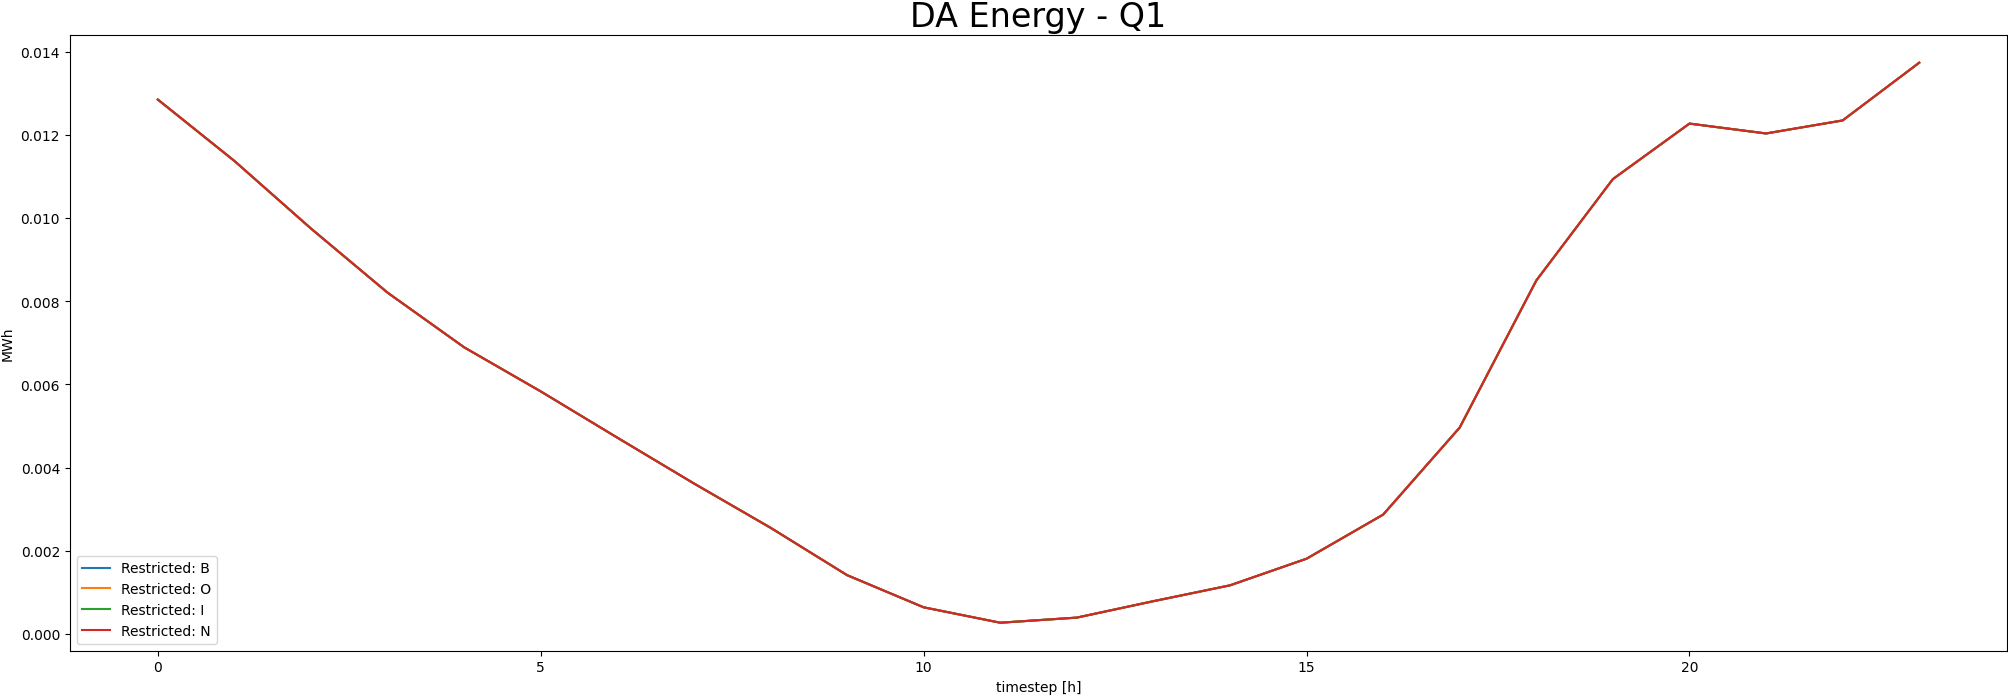
\includegraphics[width=1\linewidth]{pictures/results/DA Energy - Q1.png}
	\caption{Balance Capacity - Q1}
	\label{fig:Balance Capacity - Q1}
\end{figure}

\begin{figure}[H]
	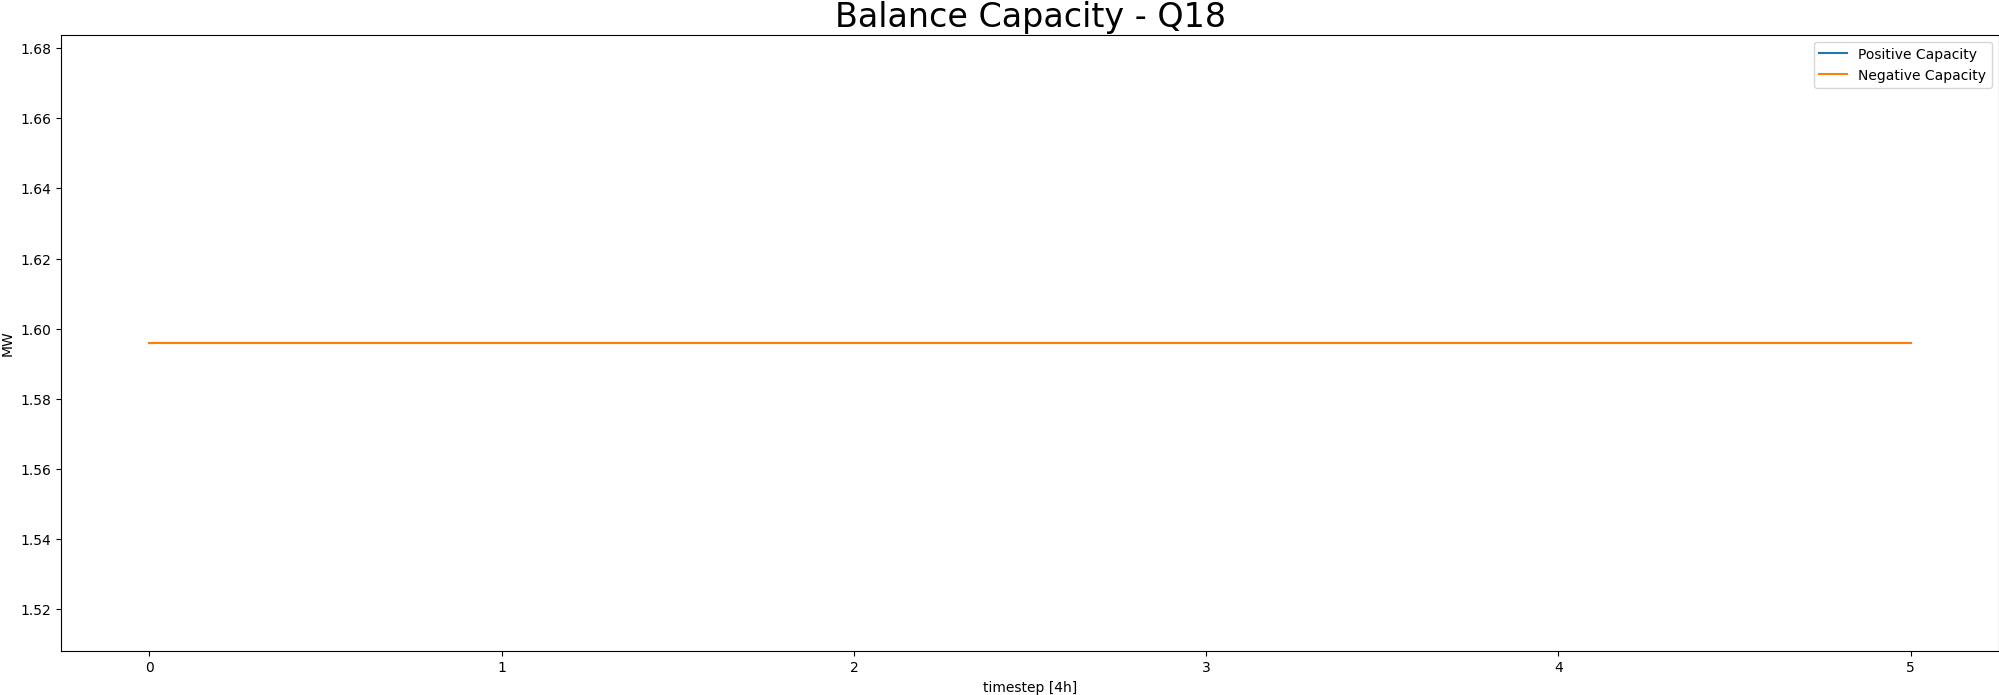
\includegraphics[width=1\linewidth]{pictures/results/Balance Capacity - Q18.png}
	\caption{Balance Capacity - Q18}
	\label{fig:Balance Capacity - Q18}
\end{figure}

\begin{figure}[H]
	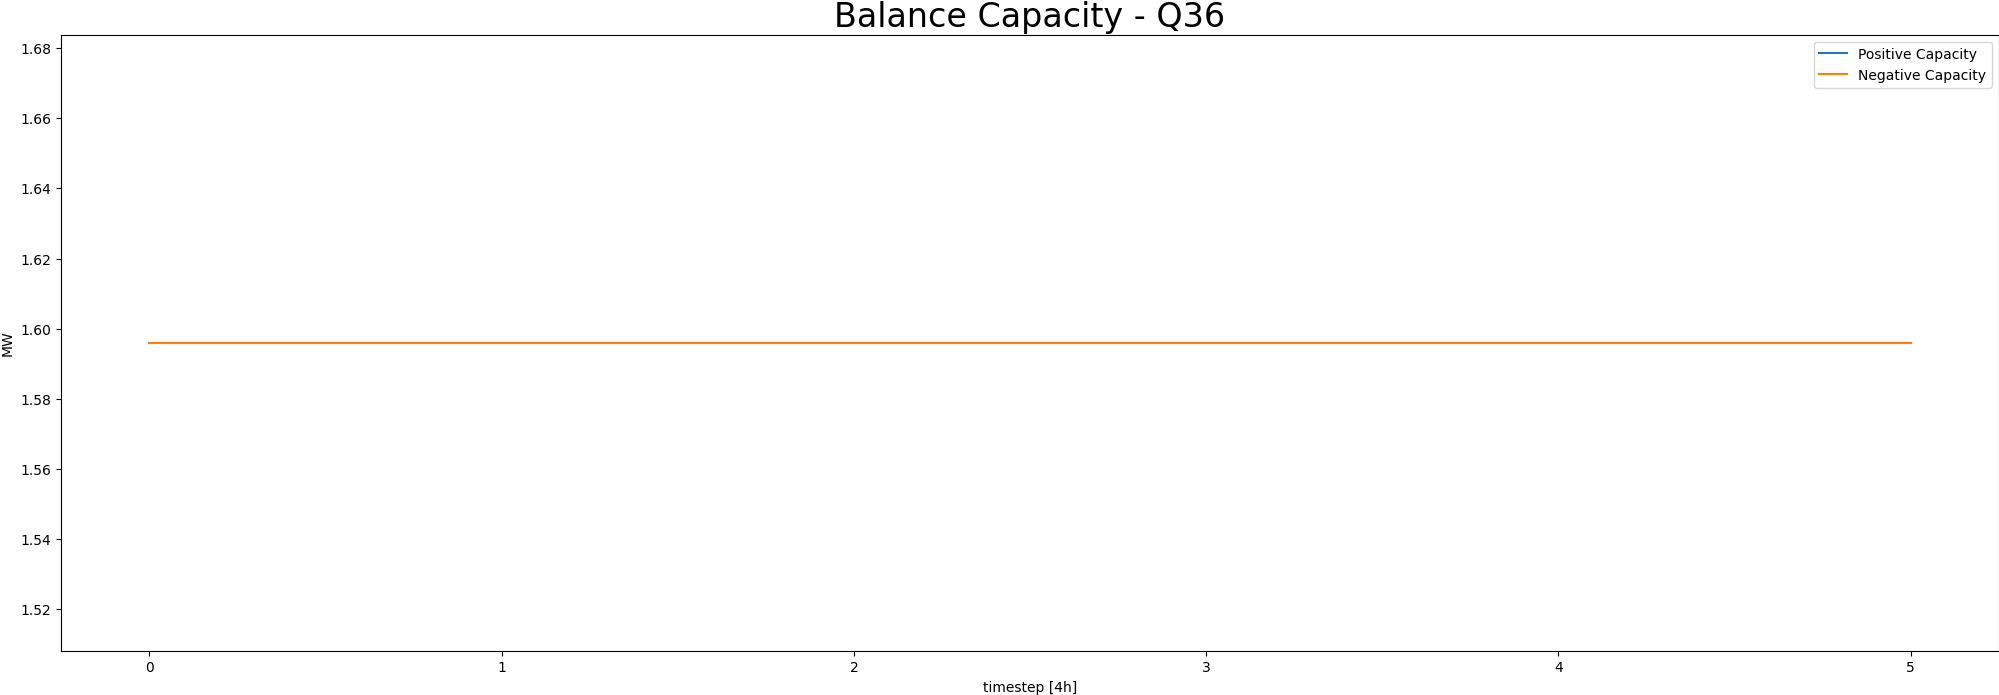
\includegraphics[width=1\linewidth]{pictures/results/Balance Capacity - Q36.png}
	\caption{Balance Capacity - Q36}
	\label{fig:Balance Capacity - Q36}
\end{figure}







\section{Digital Appendix}


